% Created 2019-09-10 Tue 14:55
% Intended LaTeX compiler: pdflatex
\documentclass[11pt]{article}
\usepackage[utf8x]{inputenc}
\usepackage[T1]{fontenc}
\usepackage{graphicx}
\usepackage{grffile}
\usepackage{longtable}
\usepackage{wrapfig}
\usepackage{rotating}
\usepackage[normalem]{ulem}
\usepackage{amsmath}
\usepackage{textcomp}
\usepackage{amssymb}
\usepackage{capt-of}
\usepackage{hyperref}
\setlength\parindent{0pt}
\setlength\parindent{0pt}
\usepackage{placeins}
\usepackage[french, english]{babel}
\newcommand{\hsp}{\hspace{20pt}}
\newcommand{\HRule}{\rule{\linewidth}{0.5mm}}
\selectlanguage{french}
\author{Billal Boudjoghra}
\date{\today}
\title{Mémoire}
\hypersetup{
 pdfauthor={Billal Boudjoghra},
 pdftitle={Mémoire},
 pdfkeywords={},
 pdfsubject={},
 pdfcreator={Emacs 26.3 (Org mode 9.1.9)}, 
 pdflang={English}}
\begin{document}
\renewcommand{\contentsname}{Table des Matières}
\begin{titlepage}
  \begin{center}

    \textsc{\LARGE Université Paris 8}\\[2cm]

    \textsc{\Large Mémoire}\\[1.5cm]

    % Title
    \HRule \\[0.4cm]
    { \huge \bfseries Détection de replays dans les vidéos\\[0.4cm] }

    \HRule \\[2cm]
    \includegraphics[scale=0.2]{paris8.png}
    \\[2cm]

    % Author and supervisor
    \begin{minipage}{0.4\textwidth}
      \begin{flushleft} \large
        Billal \textsc{Boudjoghra}
      \end{flushleft}
    \end{minipage}
    \begin{minipage}{0.34\textwidth}
      \begin{flushright} \large
        \emph{Tuteur à l'université:} M. Larbi \textsc{Boubchir}\\
        \emph{Tuteur d'alternance:} M. Régis \textsc{Jean-Gilles}
      \end{flushright}
    \end{minipage}

  \end{center}
\end{titlepage}
\tableofcontents

\newpage
\section{Sportagraph}
\label{sec:org62c3360}
Sportagraph est une start-up filiale de Everspeed, fondée en 2013 et lancée en 2016 après trois années de recherche et développement (R\&D).\\
Son produit est un DAM (Digital Asset Manager) spécialisé dans les événements sportifs.\\

Le DAM permet aux utilisateurs de stocker et de gérer plusieurs types de fichiers (principalement des images, mais les vidéos et d’autres types sont aussi supportés).\\
L’équipe travaillant sur ce projet est composée de :\\
\begin{itemize}
\item Alex Macris : Chief Experience Officer\\
\item Edouard Binchet : Chief Strategy and Operation Officer\\
\item Régis Jean-Gilles : Lead Server Developer (mon tuteur d'alternance)\\
\item Benoit Hozjan : SaaS operation manager\\
\item Francois Jacquier : Lead Developer Front\\
\item Khedidja Almherabet : Operation manager\\
\item Mate Gyomrei : Développeur front-end\\
\item Daniel Denke : Développeur iOS\\
\item Zoltan Tarsoly : Test Automation Engineer\\
\item Youva Ammaouche : Assistant chef de projet\\
\end{itemize}

En tant que développeur back end, je suis chargé de rajouter de nouvelles fonctionnalités au DAM.\\
L'une des missions qui m'a été affectée est la détection des replays dans les vidéos de sport.\\
Cette fonctionnalité permettra de fournir à nos clients un résumé automatique des vidéos qu'ils publient sur notre plateforme.\\

\newpage
\section{Introduction}
\label{sec:org1b0f66d}
Au cours des dernières années, les techniques d'apprentissage automatique ont joué un rôle de plus en plus important dans les systèmes de reconnaissance automatique.\\
Les avancements dans le domaine de l'apprentissage profond et l'accès à un volume massif de données ont permi de mettre en place des solutions de plus en plus performantes.\\
En particulier, l'adoption globale des téléphones intelligents et de leur caméra intégrée a accru de manière exponentielle le nombre de vidéos disponibles sur Internet, à tel point qu'il est devenu impossible pour l'humain d'ingérer manuellement le contenu de toutes les vidéos disponibles sur la toile.\\
Dans cette étude, nous nous intéressons à la tâche de "video summarization" ou, en français, de récapitulation de vidéo.\\
Plus particulièrement, nous focalisons notre recherche sur les vidéos de football.\\

Dans ces vidéos, notre objectif va être de parvenir à identifier les replays; car à partir de ces replays, nous serons capables de mettre en avant les moments importants du match.\\

\textbf{Qu'est-ce qu'un replay ?} Un replay est la retransmission d'une action qui s'est déjà passée au cours d'une vidéo.\\
Les replays sont intéressants car ils sont un indicateur d'un moment fort dans une vidéo.\\
En effet, c'est l'équipe technique chargée du montage de la vidéo qui décide ou non de créer un replay pour une action. Un replay est une annotation humaine sur une vidéo.\\
Typiquement, un replay sera incrusté dans la vidéo après une action importante comme, par exemple, un but ou un pénalty.\\

\textbf{Caractéristique des replays} Les replays sont introduits et se terminent par un logo (\cite{Hao_Pan_2002}).\\
Ces logos ont en général une apparence qui se démarque facilement des autres images dans la vidéo.\\
Les replays ne sont pas à confondre avec les ralentis.\\
Les ralentis sont un type particulier de replays où l'action est montrée de nouveau en \emph{slow-motion}, mais tous les replays ne sont pas des ralentis.\\
C'est pourquoi, la vitesse de déplacement des objets dans l'image (pour détecter l'effet de \emph{slow-motion}) n'est pas un bon critère pour la détection de replay.\\

L'objectif de notre recherche est de créer un système robuste de détection de replays dans les vidéos de football.\\
Dans un premier temps, nous dressons un inventaire de l'état de l'art concernant la détection de replays, puis nous présentons des méthodes par apprentissage profond pour la reconnaissance d'action dans les vidéos.\\
Une fois les bases théoriques posées, nous proposons quatre approches :\\
\begin{itemize}
\item la première utilise l'algorithme ORB \cite{Rublee_2011} pour extraire des caractéristiques à partir des images de la vidéo et K-Means à partir de ces caractéristiques\\
\item dans la seconde, nous utilisons la détection de contours pour trouver les replays\\
\item dans la troisième, nous nous servons d'un réseau à convolution 3D pour classifier des séquences d'images représentant des morceaux de la vidéo\\
\item et enfin, dans la dernière approche, nous présentons un réseau à convolution 3D qui va apprendre à classifier à partir de séquences d'images de flux optique\\
\end{itemize}
Pour conclure cette étude, nous comparons les résultats obtenus pour déterminer quelle méthode répond le mieux à notre besoin.\\

\newpage
\section{Analyse d'image : état de l'art concernant la détection de replay}
\label{sec:org03511db}
La détection de replays est un domaine de recherche à part entière et les articles sont abondants (\cite{Hao_Pan_2002,Ling_Yu_Duan,Chu_2015,Javed_2019} \ldots{}).\\
Dans cette partie, nous présentons quelques approches que nous trouvons intéressantes.\\

\subsection{Automatic Detection Of Replay Segments In Broadcast Sports Programs By Detection Of Logos In Scene Transitions}
\label{sec:org893bcaf}
\begin{figure}[htbp]
\centering
\includegraphics[width=10cm]{logo_transition.png}
\caption{Exemple de transition logo \label{logo-transition}}
\end{figure}

Dans cet article (\cite{Hao_Pan_2002}), Pan propose de détecter les replays dans les vidéos de sport en trouvant les frames contenant des logos.\\
L'auteur fait l'hypothèse que dans les vidéos de sport, les replays sont toujours compris entre deux animations spéciales qui font la transition entre le replay et le temps réel.\\
Ces transitions contiennent en général le logo de la chaîne émettant la vidéo ou de l'organisme en charge de l'événement sportif. Un montage spécifique est associé au logo.\\
Un exemple d'une de ces transitions est donné dans la figure \ref{logo-transition}. Nous voyons que le montage du logo est incrusté dans la vidéo et se déroule sur plusieurs frames; de plus, sa forme est facilement reconnaissable par rapport aux autres objets.\\
Une autre hypothèse formulée par l'auteur est que ces transitions sont les mêmes tout au long de la vidéo.\\
À partir de ces deux hypothèses, les auteurs proposent un système permettant de détecter les replays. L'idée est de trouver dans la vidéo un \emph{logo template} (pour ça, il propose d'utiliser un détecteur de \emph{slow-motion} \cite{panil_detec}), puis de trouver tous les logos dans la vidéo grâce au \emph{logo template} et à une mesure de comparaison entre une frame et le \emph{logo template}, puis finalement d'identifier les replays en regroupant les logos deux à deux.\\

Nous trouvons cette approche intéressante car elle donne un critère puissant permettant de détecter les replays : ceux-ci commencent et se terminent par une transition de logo.\\
\subsection{A Robust Replay Detection}
\label{sec:orgfb1fe4e}
Cette approche \cite{xu11_robus_replay_detec_algor_soccer_video} s'inspire de la méthode introduite par Pan et al. (\cite{Hao_Pan_2002}), et détecte les replays en trouvant les logos dans les vidéo.\\
Les logos sont trouvés grâce à la luminance. Nous savons qu'un logo est présent pendant 0.8 secondes soit 18 frames pour une vidéo de 24 FPS.\\
Toutes les frames qui ont obtenues un score supérieur à un certain seuil sont considérés comme des candidats pour être le \emph{logo template}.\\
Le \emph{logo template} est le logo qui représente le mieux les logos dans la vidéo et c'est celui-ci qui va servir de référence pour trouver tous les logos.\\

\subsubsection{Calcul du score de la luminance et filtrage des frames}
\label{sec:org4cb8c61}
L'idée est de parcourir toute la vidéo et de calculer pour chaque frame la différence de luminance qu'il y a entre cette frame et les 17 frames précédentes.\\
Nous obtenons un score L\(_{\text{i}}\) pour chaque frame i dans la vidéo.\\
Toutes les frames dont le score est inférieur à un certain seuil sont écartés, les autres vont servir à trouver le logo template.\\

\subsubsection{Recherche du logo template parmi les frames filtrées}
\label{sec:org83e2257}
Le logo template est le frame qui représente le mieux tous les logos dans la vidéo.\\
Pour déterminer le logo template parmi les frames filtrées, l'algorithme K-means est utilisé pour séparer cet ensemble en deux (K = 2) en fonction de la luminance moyenne des frames.\\
Pour trouver le logo template, il faut d'abord trouver le cluster qui contient les logos. Les auteurs estiment que c'est le cluster avec le centre det cluster le plus élevé.\\
Une fois le cluster de logos déterminé, le \emph{logo template} est la frame m qui minimise la distance avec toutes les autres frames du cluster. La formule qui permet de calculer la distance est donnée en \ref{calc-dist}.\\

\begin{figure}[htbp]
\centering
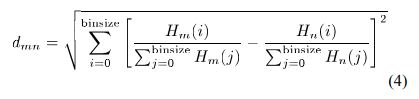
\includegraphics[width=10cm]{robust_calc_dist.JPG}
\caption{Formule de la distance entre deux frames dans le cluster \label{calc-dist}}
\end{figure}

\subsubsection{Recherche des logo}
\label{sec:org921adda}
Une fois que le logo template est déterminé, chaque logo trouvé précédemment va être comparé avec le logo template.\\
La mesure de comparaison est la distance (figure \ref{calc-dist}) qu'il y a entre le frame et le template dans le cluster.\\
Tous les frames qui ont une distance inférieure à un certain threshold sont considérés comme des logos.\\

\subsubsection{Recherche des replays}
\label{sec:orga239b19}
Une fois que les logos sont détectés, nous pouvons trouver les replays en cherchant les paires de logos éloignés de moins de 80 seconde (durée maximum d'un replay).\\

\subsubsection{Résultats obtenus et conclusion sur cette méthode}
\label{sec:org98ca862}
\begin{center}
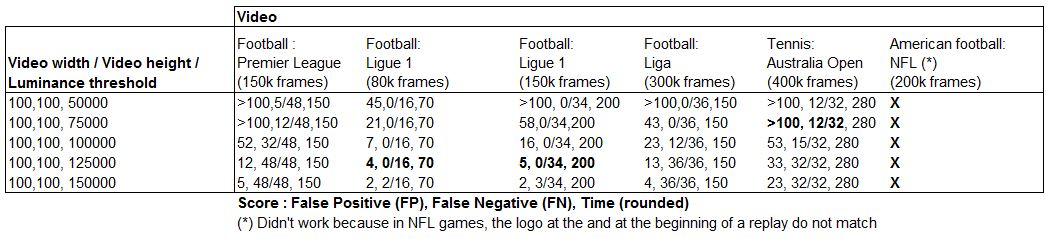
\includegraphics[width=15cm]{robust_res.JPG}
\end{center}
Après avoir implémenté cette méthode, nous avons constaté que celle-ci n'est pas efficace et ne fonctionne pas du tout sur notre ensemble de test.\\
Cette approche est trop dépendante de la luminance et elle ne parvient pas à détecter les logos peu lumineux.\\
De plus, les bases mathématiques (notamment la manière de choisir le cluster et la mesure de distance) sont un peu douteuses.\\
Enfin, celle-ci dépend trop du paramètre "seuil de luminance" affectant les logos détectés.\\
Le seuil de luminance fourni par les auteurs ne produit pas de bons résultats sur toutes les vidéos.\\
Nous n'avons pas réussi à trouver une valeur pour le seuil de luminance qui obtienne universellement de bons résultats.\\
Un seuil à 100000 détecte les logos de Ligue 1 mais pas les logos de Liga.\\
Un seuil de 75000 détecte les logos de Liga et de Ligue 1, mais laisse passer trop de faux positifs.\\
Les logos de Premier League quant à eux ne sont pas tous détectés avec un seuil à 50000, alors que ce seuil accepte un grand nombre de faux positifs.\\

Pour conclure, cette approche n'est pas celle qui va nous permettre de mettre en place un système de détection de replays robuste et efficace. Néanmoins, cet article nous a renforcé dans notre idée qu'une solution basée sur l'analyse d'image peut obtenir de bons résultats.\\

\subsection{Mean Shift Based video Segment Representation And Applications To Replay Detection}
\label{sec:orgb3851d0}
Dans cet article \cite{Ling_Yu_Duan}, les auteurs présentent une méthode permettant de détecter les replays.\\
L'idée est d'apprendre une base de représentation compressée de logos avec une méthode comme le spectral hashing (\cite{NIPS2008_3383}), puis de se servir de cette base de données pour trouver les logos au début à la fin de replays.\\
\subsubsection{Algorithme}
\label{sec:org3a9674e}
\begin{verbatim}
L = []
R = []
Segmenter la vidéo en frame
Pour chaque frame f
  Calculer la représentation r_f de f
  Pour chaque représentation r dans la base de représentation:
    Si distance(r_f, r) < Seuil:
      Ajouter f à L
Pour chaque logo l dans L:
  Trouver le logo l' lui correspondant
  Ajouter (l, l') à R
\end{verbatim}
La représentation des images est un hash obtenu par un algorithme de hashing d'image (spectral hashing).\\
La distance utilisée pour comparer le hash des images est la distance de Wasserstein .\\

\subsubsection{Résultats}
\label{sec:org494aa92}
\begin{figure}[htbp]
\centering
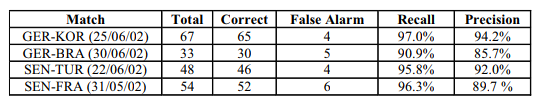
\includegraphics[width=.9\linewidth]{mean_shift_res.png}
\caption{Performance sur la tâche de détection de replay \label{mean-shift-res}}
\end{figure}
Les résultats obtenus par les auteurs sont présentés dans la Figure \ref{mean-shift-res}.\\
Ceux-ci sont bons, mais l'ensemble de test n'est pas assez représentatif (seulement quatres vidéos).\\
Les avantages des représentations hashées pour les images sont les suivants :\\
\begin{itemize}
\item un hash est compacte (peu d'espace nécessaire pour les stocker)\\
\item comparer des hash est rapide (comparer deux frames)\\
\item chercher un hash dans une table de hachage est rapide (chercher un frame dans une base de données)\\
\end{itemize}
Pour ces raisons, cette approche est tout à fait adaptée à la reconnaissance de logo.\\

\subsection{Automatic summarization of soccer highlights using audio-visual descriptors}
\label{sec:orgc8c47da}
Cette approche \cite{Ravent_s_2015} ressemble à l'approche par luminance (\cite{xu11_robus_replay_detec_algor_soccer_video}), mais introduit néanmoins une différence importante : un pré-traitement sur la vidéo pour en extraire les plans.\\
\subsubsection{Algorithme}
\label{sec:orga39ba0d}
L'algorithme est le suivant :\\
\begin{verbatim}
S = Détecter tous les shots (plans) dans la vidéo
L = Pour chaque shot S_i:
1. L_i_start = La "luminance" des frames au début du shot
2. L_i_end = La "luminance" des frames à la fin du shot
3. L_template = Trouver le "logo template" dans L
4. Pour chaque logo l dans L:
   1. Diff l avec L_template = conversion grayscale puis somme de la soustraction pixel par pixel
   2. Si Diff l avec L_template < threshold => l est un logo
\end{verbatim}

\subsubsection{Apport de l'article}
\label{sec:org4d1a79c}
Cette méthode est trop semblable à l’approche “Robust Replay Detection” qui ne répond pas à nos besoins, cette approche ne fonctionnera pas dans notre cas (la luminance n’est pas un critère assez discriminant pour la reconnaissance de logo).\\
Néanmoins, l’idée de découper la vidéo en “shot” (en plan) est intéressante et nous nous en servons par la suite.\\

\newpage
\section{Apprentissage automatique : les bases théoriques}
\label{sec:orgfa11581}
Dans notre recherche, nous allons aborder plusieurs types de réseaux d'apprentissage automatique.\\
Nous allons présenter dans cette partie les principes fondamentaux à la bonne compréhension de ces derniers.\\

\subsection{Réseaux de neurones récurrents (RNN)}
\label{sec:org1eaf634}
Les RNN (Recurrent Neural Networks), ou réseaux de neurones récurrents (RNR) en français, sont capables de répéter leur couche cachée, en utilisant comme entrée la sortie de toutes les couches précédentes et de générer une sortie pour chaque couche.\\
Cela va leur permettre de prendre en entrée des séquences et de retourner des séquences.\\
En effet, pour une entrée [e\(_{\text{1}}\), e\(_{\text{2}}\),\ldots{}, e\(_{\text{n}}\)] et un initialiseur s\(_{\text{0}}\), le RNN va répéter n fois sa couche cachée, de telle sorte à générer une sortie s\(_{\text{1}}\) associée à la couche 1 et à l'entrée (e\(_{\text{1}}\), s\(_{\text{0}}\)); puis il va générer une sortie s\(_{\text{2}}\) associée à la couche 2 et à l'entrée (e\(_{\text{2}}\), s\(_{\text{1}}\)), etc \ldots{}\\
Pour finir, nous aurons en sortie la séquence [s\(_{\text{1}}\), s\(_{\text{2}}\), \ldots{}, s\(_{\text{n}}\)].\\

Par exemple, appliqués à la génération de phrase, les RNN vont être capables de générer (mot par mot, ou n-gram par n-gram) des séquences de phrases de longueur arbitraire.\\

Pour apprendre un modèle, le RNN va avoir besoin d'un ensemble d'entraînement qui met en avant les propriétés qui nous intéressent dans le modèle.\\

La nature récursive de ces réseaux les rend particulièrement adaptés aux tâches de traitement du langage naturel ou pour traiter la temporalité (ce qui nous intéresse car la temporalité est ce qui différencie l'analyse d'images à l'analyse vidéo).\\

\subsection{LSTM}
\label{sec:orgacadfde}
Les LSTM (Long Short Term Memory) sont un type de RNN \textbf{à portes (gated RNN)}.\\
Ces portes vont permettre de stocker l'information apprise par le réseau à travers le temps.\\
À la différence des RNN classiques, les LSTM sont capables d'oublier de l'information grâce à leur \textbf{leaky unit} afin d'éviter une explosion ou une disparition du gradient.\\
Par exemple, si nous voulons entraîner un LSTM pour qu'il puisse reconnaître une action courte dans une vidéo, ce dernier n'a pas besoin d'enregistrer toutes l'information acquise depuis le premier frame, il lui suffit de connaître un voisinage de quelques frames.\\
La puissance de ces réseaux à portes est que c'est le réseau qui va apprendre à décider quand vider son état interne.\\
Concrètement, cela va leur permettre de pouvoir capturer des dépendances à long terme de manière bien plus efficace que les RNN classiques.\\

\subsection{CNN}
\label{sec:org452284e}
\begin{figure}[htbp]
\centering
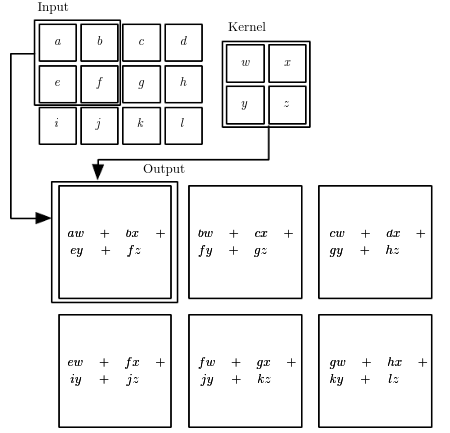
\includegraphics[width=7cm]{convolution.png}
\caption{Opération de convolution \label{convolution}}
\end{figure}
Les CNN (Convolutional Neural Networks), ou réseaux de neurones convolutifs (RNC) en français, sont un type de réseau de neurones qui utilisent la convolution au lieu de la multiplication matricielle dans au moins une de leurs couches.\\
La convolution est une opération qui prend en argument l'entrée (typiquement un vecteur représentant une donnée) et un \textbf{noyau} (les paramètres qui vont être appris par le CNN) et renvoie une \textbf{carte de caractéristiques} (feature map).\\
Le noyau est une matrice qui va parcourir l'entrée et appliquer l'opération de convolution.\\
Pour parcourir l'entrée, celle-ci va être divisée en plusieurs matrices carrées de même taille que le noyau (par exemple 2x2 ou 6x6) en ajoutant si nécessaire du \emph{padding} et du \emph{striding}.\\
La fonction de convolution a trois caractéristiques importantes : l'\textbf{intéraction parcimonieuse} ("sparse interaction"), le \textbf{partage de paramètres} et les \textbf{représentations équivariantes}.\\
La couche de convolution est généralement composée de la fonction de convolution suivie d'une fonction d'activation non linéaire (par exemple, ReLU ou tanh) et d'une d'une fonction de \textbf{pooling}.\\

\subsubsection{Intéraction parcimonieuse}
\label{sec:org310c5e7}
\begin{figure}[htbp]
\centering
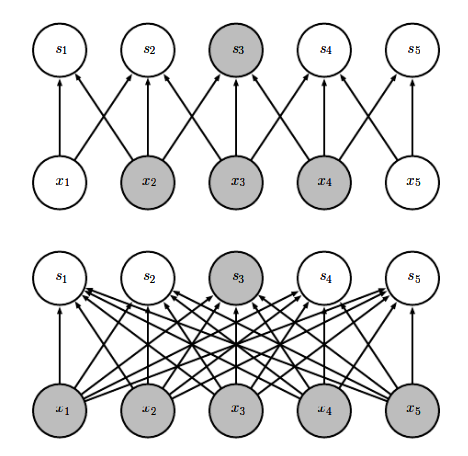
\includegraphics[width=8cm]{sparse_vs_dense.png}
\caption{Intéraction parcimonieuse (en haut), intéraction non parcimonieuse (en bas) \label{sparse-vs-dense}}
\end{figure}

À la différence des réseaux classiques où toutes les sorties intéragissent avec toutes les entrées, les réseaux à convolution ont des \textbf{intéractions parcimonieuses}.\\
C'est-à-dire que la taille du noyau (donc de l'intéraction avec l'entrée), est plus petite que la taille de l'entrée.\\
Une image a une dimension en entrée de \emph{c*l*w} où \emph{c} est le nombre de canaux de l'image (un seul pour une image en noir et blanc, trois pour une image en couleur), l la largeur en pixel de l'image et w la longueur en pixel de l'image.\\
Une petite image couleur de dimension 100*100 aura 100*100*3 paramètres en entrée, ce qui provoque une explosion combinatoire avec les réseaux classiques qui n'ont pas d'intéraction parcimonieuse car il faudra une connexion entre chaque paramètre d'entrée et une entrée du réseau.\\
Un réseau de convolution, quant à lui, aura un noyau d'une dizaine ou d'une centaine de pixel qui parcourt l'image à la recherche de caractéristiques significatives comme des contours.\\
Cela signifie que l'intéraction parcimonieuse permet aux CNN de stocker moins de paramètres que les autres types de réseau.\\
Par conséquent, ils ont donc ont besoin de moins de mémoire (pour la même tâche) et ont une meilleure efficacité statistique.\\
C'est l'une des raisons faisant que les réseaux à convolution sont très efficaces pour le traitement d'image.\\

\subsubsection{Partage de paramètres}
\label{sec:org155f20c}
Dans un réseau classique, un poids (un paramètre) est associé à chaque paramètre d'entrée et ne sert qu'une fois.\\
Tandis que dans un réseau convolutif, le noyau utilisé par une couche de convolution est le même sur toutes les matrices représentant l'entrée.\\
Grâce à ce \textbf{partage des paramètres}, il n'y a que les poids du noyau à apprendre au lieu d'un poids pour chaque neurone d'entrée.\\
De plus, la taille du noyau est en général largement inférieure à celle de la couche d'entrée.\\

\subsubsection{Représentations équivariantes}
\label{sec:orgd193a52}
Une fonction est \textbf{équivariante} si, quand l'entrée change, la sortie change de la même manière.\\
En terme mathématique, cela signifie que si \(y = f(x)\) alors \(g(y) = g(f(x))\).\\
Les réseaux convolutifs sont équivariants à la translation.\\
Dans le cas de l'image, cela veut dire que le déplacement des pixels n'a pas d'influence sur le réseau.\\

\subsubsection{Pooling}
\label{sec:orgdc15c6b}
\begin{figure}[htbp]
\centering
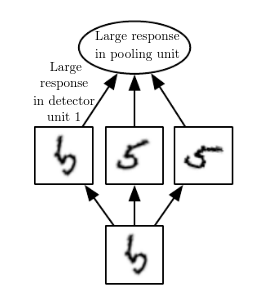
\includegraphics[width=8cm]{pooling.png}
\caption{Pooling \& invariance \label{pooling}}
\end{figure}
La fonction de pooling va modifier la sortie de la couche de convolution.\\
Pour chaque valeur dans la carte des caractéristiques à la sortie de la convolution (après la fonction d'activation), la fonction de pooling va remplacer celle-ci en fonction de la valeur des cases voisines dans la carte.\\
Une fonction de pooling usuelle est max pooling, qui va renvoyer la plus grande valeur dans un voisinage rectangulaire.\\
L'utilité de la fonction de pooling est de rendre la représentation apprise par la couche de convolution \textbf{invariante} à de petites modifications sur l'entrée.\\
Par exemple, dans le cas de la reconnaissance d'image, le réseau ne va pas chercher dans l'image en entrée les informations au pixel près.\\
Si le réseau a appris à détecter les visages, il n'a pas besoin de retrouver l'emplacement des yeux au pixel près, une position approximative de ceux-ci lui suffira.\\
Une autre utilité du pooling est de réduire la taille de la sortie de la couche de convolution.\\
Nous pouvons voir le pooling comme un résumé de la carte des caractéristiques obtenue par convolution.\\

\newpage
\section{Apprentissage profond : état de l'art pour la reconnaissance d'action dans les vidéos}
\label{sec:org1c221af}
Nous nous intéressons à l'état de l'art concernant la détection d'action dans les vidéos.\\
En effet, la transition d'un logo s'effectue sur plusieurs frames consécutifs; il y a donc une composante temporelle à notre recherche, et nous pouvons considérer la transition d'un logo comme une action.\\

\subsection{Two-Stream Convolutional Networks for Action Recognition in Videos}
\label{sec:orgf3356c9}
Cet article est écrit par Karen Simonyan et Andrew Zisserman \cite{DBLP:journals/corr/SimonyanZ14}. Dans celui-ci, ils proposent de séparer la tâche de reconnaissance d'action dans les vidéos en deux parties : une composante spatiale et une composante temporelle.\\

La composante spatiale contient l'information concernant les objets dans la vidéo; tandis que la composante temporelle l'information sur les déplacements de ces objets et de la caméra.\\
A partir de ces observations, les auteurs proposent d'entraîner un classifieur spatial (Spatial stream ConvNet) et un classifieur temporel (Temporal stream ConvNet).\\

Ces classifieurs sont des réseaux de neurones convolutifs profonds.\\

\subsubsection{Classifieur spatial}
\label{sec:orgedab299}
Ce réseau a une architecture de classifieur d'image classique.\\
Il va permettre de donner un indice fort pour la prédiction, car certaines actions sont très liées à certains objets.\\
De plus, la recherche dans le domaine de la classification est un domaine à part entière; toutes les avancées dans le domaine augmenteront l'efficacité de ce classifieur.\\
Il n'est pas nécessaire d'apprendre ce réseau "from scratch" (de zéro), les approches par \emph{transfer learning} sont efficaces.\\

\subsubsection{Classifieur temporel}
\label{sec:orgac7e7cf}
\begin{figure}[htbp]
\centering
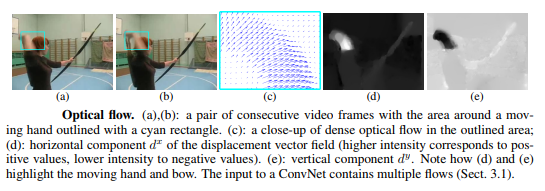
\includegraphics[width=12cm]{optical_flow.png}
\caption{Flux optique \label{optical-flow} \label{opt-flow}}
\end{figure}
L'innovation de l'article vient de l'introduction du classifieur temporel.\\

L'idée est de détecter le mouvement des objets dans la vidéo, car un mouvement est la représentation d'un objet dans le temps.\\
Les auteurs appellent leur approche "optical flow stacking" (empilement de flux optique).\\

Dans celle-ci, ils utilisent le flux optique pour représenter le mouvement des objets entre des frames consécutifs.\\

Ils définissent aussi un hyperparamètre L qui définit la distance maximum entre deux frames pour laquelle il faut calculer le flux optique.\\
Par exemple, si L=5, alors pour le frame t, il faudra calculer le flux entre le frame t et le frame t+1; entre t+1 et t+2; etc\ldots{} jusqu'à t+4 et t+5.\\
Le flux optique entre deux frames est une matrice de dimension 2, il peut donc être sauvegardé sous forme d'image.\\
Ainsi, des images représentant le flux optique entre les différents frames de la vidéo vont être générées.\\

Chacune de ces images servira d'entrée au CNN (classifieur temporel).\\
\subsubsection{Méthode d'évalutation et résultats obtenus}
\label{sec:org870ade7}
\begin{figure}[htbp]
\centering
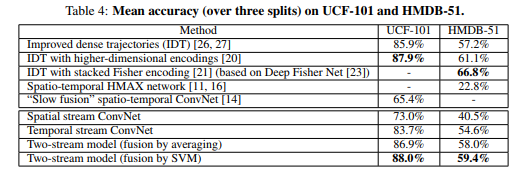
\includegraphics[width=13cm]{two_stream_res.png}
\caption{Résultats obtenus par l'approche Two-stream model \label{two-stream-res}}
\end{figure}

Le classifieur spatial est pré-entrainé avec ImageNet, tandis que le temporel est entraîné de zéro (car il n'y a pas de réseau déjà entraîné pour cette tâche).\\
Les ensemble de données utilisés pour l'entraînement et l'évaluation sont UCF-101 et HMDB-51, contenant à eux deux près de 20000 vidéos annotées.\\
Avant l'entraînement, les images de flux optiques sont pré-calculées afin de n'avoir à générer ces images qu'une seule fois.\\

\textbf{Note} Pour calculer la classe d'un frame à l'instant t, les auteurs proposent deux méthodes :\\
\begin{itemize}
\item fusion par la moyenne (by averaging) : y\(_{\text{t}}\) = y\(_{\text{t}}\)\(_{\text{spatial}}\) + y\(_{\text{t}}\)\(_{\text{temporal}}\) / 2\\
\item fusion par SVM (by SVM) : un SVM multiclasse linéaire est entrainé pour prédire la classe à partir du softmax des scores L2-normalisés.\\
\end{itemize}

Les résultats (figure \ref{two-stream-res}) montrent l'efficacité de leur méthode par rapport aux autres approches état de l'art.\\

Nous pouvons voir que leur approche two-stream avec fusion SVM est la plus efficace sur le dataset UCF-101, et qu'elle a aussi de bons résultats sur HMDB-51.\\

Ce qui est le plus intéressant dans cet article, c'est l'amélioration qu'apporte l'ajout de la composante temporelle.\\
En effet, le classifieur d'image simple (spatial) n'a que 73.0\% (UCF-101) et 40.5\% (HMBD-51), tandis que le classifieur qui prend en compte l'image et la temporalité (two-stream model) atteint \textbf{88.0\%} et 59.4\%; ce qui est une nette amélioration.\\

Cet article nous a renforcés dans l'hypothèse qu'il est nécessaire d'étudier une vidéo non pas comme une suite d'images indépendantes, mais comme une suite de séquences avec un lien entre chaque élément de la séquence. La temporalité a une très grande importance pour l'analyse de vidéos, et le flux optique est une méthode efficace pour modéliser le déplacement des objets entre deux instants.\\

\subsection{Learning Spatiotemporal Features with 3D Convolutional Networks}
\label{sec:orgaeba9bd}
Dans cet article \cite{Tran_2015}, les auteurs proposent une approche pour apprendre les caractéristiques spatio-temporelles dans les vidéos grâce à un réseau de neurones à convolution.\\

Ils font l'hypothèse qu'un réseau avec une couche de convolution 3D qui prend en entrée une séquence d'images est capable d'apprendre efficacement les mouvements des objets dans les vidéos.\\

L'objectif est d'apprendre des caractéristiques qui soient :\\
\begin{itemize}
\item génériques : c'est-à-dire la capacité à représenter différents types de vidéos\\
\item compactes : afin de pouvoir stocker un grand nombre de ces caractéristiques\\
\item efficace (computationnellement): pour traiter les vidéos en temps réel\\
\item simples : afin de fonctionner même avec les modèles simples (comme un classifieur linéaire)\\
\end{itemize}

\subsubsection{C3D: Convolution et pooling 3D}
\label{sec:org3b29f9f}
\begin{figure}[htbp]
\centering
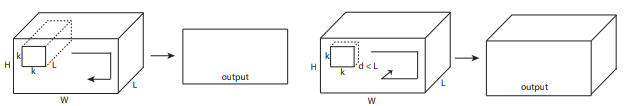
\includegraphics[width=.9\linewidth]{c3d_idea.png}
\caption{Convolution 2D sur une séquence d'images (gauche), convolution 3D sur une séquence d'images (droite) \label{c3d-idea}}
\end{figure}
Les auteurs appellent leur approche C3D (3D ConvNet).\\
Comparé aux réseaux à convolution 2D, C3D est capable de modéliser plus efficacement l'information spatio-temporelle grâce à la convolution et au pooling sur trois dimensions.\\
La convolution 2D appliquée à une image produira en sortie une image, la convolution 2D appliquée à une suite d'images produira aussi une image.\\
C'est pourquoi les réseaux à convolution 2D perdent l'information temporelle après l'opération de convolution. La convolution 3D permet, elle, de préserver cette information dans sa dimension additionnelle.\\

\subsubsection{Architecture et entraînement du réseau}
\label{sec:orge494dd3}
\begin{figure}[htbp]
\centering
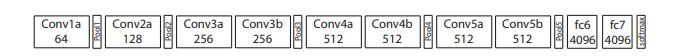
\includegraphics[width=13cm]{c3d_architecture.jpg}
\caption{Architecture C3D \label{arch-c3d}}
\end{figure}
L'entrée de ce réseau est de dimension c * l * h * w où c est le nombre de canaux des images (3 pour la couleur, 1 pour les images en noir et blanc), l le nombre d'images dans les séquences, h la longueur et w la largeur en pixel des images.\\

L'architecture conseillée par les auteurs est 8 couches de convolution et 5 couches de pooling, ainsi que 2 couches complètement connectées et la fonction softmax pour la couche de sortie.\\
Le kernel recommandé par les auteurs est 3 * 3 * 3 avec un pas (stride) de 1 * 1 * 1 pour toutes les couches de convolution.\\
Toutes les couches de pooling sont max pooling avec une taille de kernel 2 * 2 * 2 (sauf pour la première qui est 1 * 2 * 2) avec un stride 2 * 2 * 2 (sauf pour la première qui a un stride de 1 * 2 * 2).\\
Pour finir avec l'architecture, les deux couches complètement connectées ont 4096 sorties.\\

Ce réseau va être entraîné de zéro par descente du gradient à partir de séquences d'images annotées.\\
Le taux d'apprentissage est de 0.003 et est divisé par 10 toutes les 4 epoch.\\
L'entraînement s'arrête après 16 epoch.\\

Après l'entraînement, le réseau peut être utilisé comme un extracteur de caractéristiques pour des tâches d'analyse vidéo.\\
Pour se faire, la vidéo va être découpée en des clips de 16 frames (avec 8 frames de chevauchement entre deux clips consécutifs).\\
Ensuite, chacun de ces clips va être passé au réseau et l'avant dernière couche complètement connectée (fc6) va contenir les caractéristiques du clip.\\

\textbf{Qu'est-ce que ce réseau apprend ?} Ce réseau apprend à se focaliser sur l'image des premiers frames, et à traquer leur déplacement dans les frames suivants.\\

\subsubsection{Résultat pour la tâche de reconnaissance d'action}
\label{sec:org2209876}
\begin{figure}[htbp]
\centering
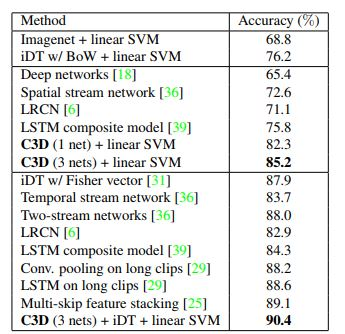
\includegraphics[width=7cm]{c3d_result.jpg}
\caption{Résultats pour l'approche Learning Spatiotemporal Features with 3D Convolutional Networks (C3D) comparés à d'autres approches état de l'art \label{c3d-res}}
\end{figure}
Ces résultats (figure \ref{c3d-res}) ont été obtenus par les auteurs pour la tâche de reconnaissance d'action sur le corpus de vidéo UCF101.\\
Nous voyons que l'approche par réseau à convolution 3D est la plus efficace.\\

\subsubsection{Conclusion}
\label{sec:org26d90d8}
Dans cet article, les auteurs ont adressé le problème de la temporalité dans les vidéos.\\
Ils ont montré qu'un réseau à convolution 3D est capable de modéliser l'information temporelle et spatiale simultanément, et donc d'obtenir de meilleurs résultats que les réseaux à convolution 2D pour l'analyse de vidéos.\\
De plus, cette approche est élégante car elle fonctionne sans ajout artificiel d'information (comme le flux optique), c'est le réseau qui va se charger d'apprendre ce dont il a besoin pour apprendre la temporalité.\\

\subsection{Beyond Short Snippets: Deep Networks for Video Classification}
\label{sec:orge5728bd}
Dans cet article \cite{Joe_Yue_Hei_Ng_2015}, les auteurs proposent d'utiliser une architecture hybride à base de CNN et de RNN (LSTM) pour l'analyse vidéo.\\
Leur objectif est d'apprendre des dépendances à long terme dans les vidéos, d'où l'utilisation d'un LSTM.\\
Les CNN sont des réseaux particulièrement efficaces pour analyser les frames des vidéos, c'est le CNN qui va se charger de la composante spatiale de la vidéo.\\
Le LSTM va servir à apprendre la composante temporelle.\\

\subsubsection{Approche}
\label{sec:org9e3423f}
L'objectif des auteurs est d'apprendre des dépendances à long terme dans les vidéos.\\
Les réseaux à convolution sont très efficaces pour l'analyse d'image; mais leur coût computationnel est très élevé.\\
C'est pourquoi, il n'est pas possible de se servir d'un CNN pour apprendre les dépendances à long terme; en effet, il faudrait que le réseau prenne en entrée toute la vidéo (ou bien une grande partie), ce qui va provoquer une explosion combinatoire des paramètres à apprendre par le réseau.\\
Les auteurs font l'hypothèse que tous les frames dans la vidéo ne sont pas utiles, et qu'il est judicieux de ne garder qu'un sous-ensemble des frames de la vidéo; ils proposent donc de ne traiter qu'un frame par seconde. L'intérêt de ne garder qu'un sous ensemble des images de la vidéo et qu'il va donc être possible de traiter la vidéo sur une plage temporelle plus large pour le même coût en calcul.\\
Néanmoins, ne regarder qu'une seule image par seconde dans la vidéo ne préserve pas le déplacement des pixels entre l'instant t et l'instant t + 1 (en seconde) et donc l'information du mouvement des objets.\\
Pour palier à ce problème, le flux optique (de la même manière que \cite{DBLP:journals/corr/SimonyanZ14}) est calculé entre les frames adjacents.\\
Ainsi, l'information temporelle et l'information spatialle sont préservées, tout en ne traitant qu'une seule image par seconde, ce qui réduit beaucoup le coût de calcul.\\
Pour apprendre les dépendances qu'il y a entre les frames, un LSTM est utilisé; celui-ci va traiter les vidéos comme des séquences d'images et va apprendre à prédire la classe de la vidéo en fonction de ces séquences.\\
\subsubsection{Architecture}
\label{sec:org5329efa}
\begin{figure}[htbp]
\centering
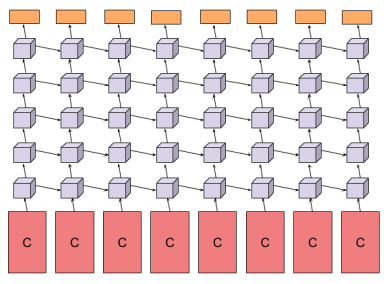
\includegraphics[width=8cm]{cnn_lstm.PNG}
\caption{Architecture du LSTM \label{arch-lstm}}
\end{figure}
Comme pour \cite{DBLP:journals/corr/SimonyanZ14}, un réseau à convolution va être utiliser pour extraire les caractéristiques visuelles de la vidéo.\\
Les architectures utilisées pour ce réseau sont GoogLeNet et AlexNet.\\

L'architecture proposée pour le LSTM est présentée en \ref{arch-lstm}.\\
La sortie du CNN est processée par propagation avant à travers cinq couches de LSTM.\\
La couche de sortie du LSTM est munie de la fonction softmax et prédit une classe à chaque étape.\\
Les paramètres du réseau à convolution et de la couche de sortie du LSTM sont partagés pour toutes les étapes.\\

\subsubsection{Utilisation du flux optique}
\label{sec:orgeeaa9f2}
Le flux optique encode l'information des déplacements des objets dans la vidéo.\\
Comme pour l'approche \cite{DBLP:journals/corr/SimonyanZ14}, les images de flux vont être pré-calculées et servir lors de l'entraînement du CNN.\\

\subsubsection{Résultat obtenu}
\label{sec:org24e7ebe}
\begin{figure}[htbp]
\centering
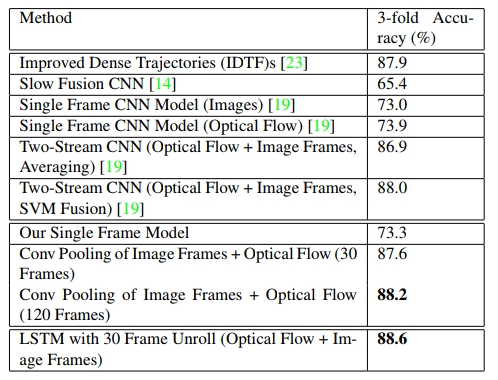
\includegraphics[width=10cm]{cnn_lstm_res.png}
\caption{Résultat obtenu pour l'approche combinant CNN et LSTM (LSTM with 30 Frame Unroll) \label{cnn_lstm}}
\end{figure}
Les auteurs évaluent leur approche sur le dataset Sports-1M et UCF-101 sur la tâche de classification de vidéos.\\
Nous pouvons voir que leur approche obtient les meilleurs résultats (88.6\% contre 88.0\% pour \cite{DBLP:journals/corr/SimonyanZ14}).\\
Ces résultats sont intéressants car à la différence des autres approches, celle-ci est capable de prédire une classe pour des morceaux de vidéos pouvant aller jusqu'à deux minutes (contre quelques secondes pour les autres).\\
De plus, les meilleurs résultats sont là aussi obtenus en utilisant le flux optique, confirmant l'hypothèse faite par \cite{DBLP:journals/corr/SimonyanZ14} que ce dernier est nécessaire pour le traitement des vidéos.\\

Dans notre cas, cette approche n'est pas la plus adaptée. En effet, nous souhaitons reconnaître les logos dans les vidéos, or un logo ne dure pas plus longtemps que quelques secondes et les dépendances à long-terme que le LSTM va apprendre ne nous intéressent pas.\\
Néanmoins, une variante de celle-ci où le LSTM reçoit en entrée une séquence de frames consécutifs (et pas une séquence formée d'un frame par seconde) pourrait avoir de bons résultats pour la tâche de détection de logos.\\

\newpage
\section{Les approches proposées}
\label{sec:org6e35a77}
L'objectif de notre recherche est de détecter les replays dans les vidéos de sport.\\

Pour détecter les replays, nous faisons les hypothèses suivantes :\\
\begin{itemize}
\item un replay a un logo de début (I) \cite{Hao_Pan_2002} \\
\item un replay a un logo de fin (II) \cite{Hao_Pan_2002}\\
\item les logos de début et de fin sont les mêmes (III) \cite{Hao_Pan_2002}\\
\item les logos ont une forme facilement reconnaissable qui se distingue des  autres images dans la vidéo (IV)\\
\item un replay dure entre 2 et 90 secondes (V)\\
\end{itemize}

En faisant ces hypothèses, la tâche de détection de replays devient une tâche de détection de logos.\\

Nous proposons plusieurs approches permettant de détecter les logos de replay dans les vidéos de sport.\\
En premier lieu, nous proposons deux approches n'utilisant que des algorithmes d'analyse d'images classiques (flouttage, filtre de Canny, ORB, \ldots{}) :\\
\begin{itemize}
\item la première se sert de l'algorithme ORB (\cite{Rublee_2011}) et de l'algorithme K-Means\\
\item la seconde utilise la détection de contours pour trouver les images avec des contours similaires dans la vidéo\\
\end{itemize}
Ensuite, nous présentons deux approches par apprentissage profond :\\
\begin{itemize}
\item la première utilise un réseau à convolution 3D sur une séquence d'images (similaire à \cite{Tran_2015})\\
\item la seconde utilise un réseau à convolution 3D sur des séquences d'images représentant le flux optique des objets dans la vidéo\\
\end{itemize}

\subsection{Détection des plans}
\label{sec:org704a801}
\begin{figure}[htbp]
\centering
\includegraphics[width=10cm]{plan.png}
\caption{Changement de plan introduit par un replay \label{plan}}
\end{figure}

Les approches que nous proposons recherche dans la vidéo les logos pouvant se trouver au début et à la fin des replays.\\
Or, un replay introduit un changement avant et après lui (car l'action rejouée par le replay n'est pas sur le même plan que l'action avant et après lui).\\
Si nous faisons l'hypothèse qu'un replay entraînera toujours un changement de plan et que les logos sont au début et à la fin du replays, alors au lieu de rechercher les logos parmi tous les frames de la vidéo, nous pouvons réduire la recherche seulement aux frames qui sont entre deux plans.\\
En effet, le logo au début du replay introduit un changement de plan entre l'action avant le replay et le replay, et le logo à la fin du replay introduit un changement de plan entre l'action après le replay et le replay. La figure \ref{plan} illustre cette hypothèse.\\

C'est pourquoi nous allons chercher une méthode permettant de détecter les changements de plan dans les vidéos.\\

\subsubsection{Online, Simultaneous Shot Boundary Detection And Key Frame Extraction For Sports Videos Using Rank Tracing}
\label{sec:org4334530}
Cette méthode est proposée par W. Abd-Almageed en 2008 \cite{Abd_Almageed_2008}.\\

Chaque frame est converti en HSV et les histogrammes H, S et V sont calculés.\\
Un vecteur est formé pour chaque frame à partir de ces histogrammes.\\
Ensuite, une matrice M de dimension N * L, représentant une fenêtre de N frames va être formée à partir de ces vecteurs, où L est la taille des histogrammes et N la taille de la fenêtre.\\

L'algorithme SVD (singular value decomposition) va être appliqué sur M.  \(M = UWV\), où W est la matrice de valeurs singulières.\\

Les diagonales de la matrice W comportent des poids S ordonnés de manière décroissante.\\
Le premier poids S\(_{\text{1}}\) est le poid maximal. Ces poids représentent l'information contenue dans le vecteur V.\\

Nous allons assigner un rang à la matrice M,  ce rang va être égal au nombre d'éléments s dans S tel que s/S1 > threshold. Le rang va être calculé pour chaque fenêtre de frames dans la vidéo.\\

Si le rang d'une fenêtre est plus grand que le rang de la fenêtre avant elle, alors le contenu visuel de la fenêtre est différent de la fenêtre précédente.\\
À l'inverse, si le rang est inférieur à la fenêtre précédente, alors le contenu visuel se stabilise. S'il est de 1, alors c'est stable.\\

Le début d'un nouveau plan est indiqué par la fenêtre qui maximise le rang parmi les fenêtres environnantes.\\

Cette méthode pour trouver les plans dans une vidéo est très efficace, et nous servira dans la suite de notre recherche.\\

En effet, avant de segmenter la vidéo en plan, nous comparions  N frames , où N peut être aussi grand que 400000 (pour des vidéos de 120 minutes à 60 fps).\\
Il est impensable d’utiliser un algorithme en O(N²), par exemple en comparant tous les frames entre eux, avec un N aussi grand.\\

Après avoir segmenté la vidéo en plan, nous obtenons un N’ aux alentours de 2000 pour une vidéo de 120 minutes à 60 fps.\\
Nous pouvons donc nous permettre d’utiliser des algorithmes plus complexes que sans la segmentation en plan.\\
De plus, la segmentation en plan réduit le champ de recherche des frames logo, et donc le nombre de faux positifs.\\

\subsection{Flux optique}
\label{sec:org239d620}
\begin{center}
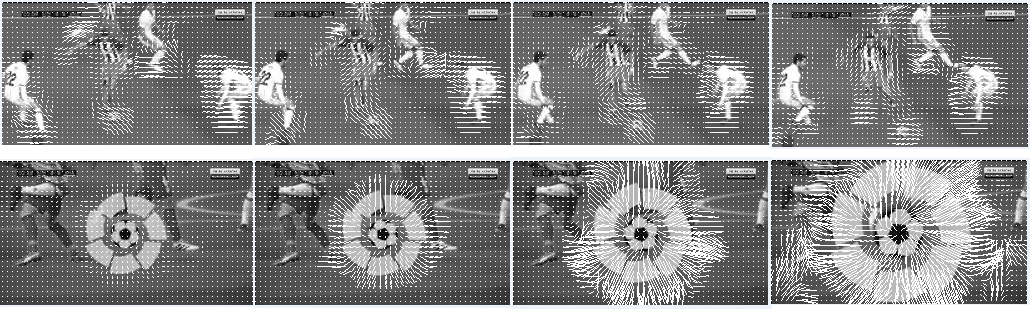
\includegraphics[width=.9\linewidth]{optical_flow_2.png}
\end{center}
Le flux optique décrit le déplacement des objets entre deux frames consécutifs, ce mouvement peut être causé par un déplacement de la caméra ou de l'objet lui-même.\\
Le flux optique est une matrice X * Y * D, où X et Y sont l'axe des absisses et des ordonnées (resp.) dans l'image, et D une droite décrivant le déplacement du pixel à la position (x,y) entre le frame t et le frame t + 1.\\

De la même manière que pour \cite{wang11_action}, nous allons traquer le déplacement des objets grâce au flux optique.\\
Il existe deux types d'algorithme de calcul du flux optique :\\
\begin{itemize}
\item sparse/creux : seulement le déplacement de certains points d'intérêt va être traqué (méthode de Lucas-Kanade)\\
\item dense : le déplacement de tous les points dans l'image va être traqué (algorithme de Gunner Farneback)\\
\end{itemize}
Le calcul du flux optique dense est plus couteux mais à l'avantage de ne pas nécessiter de déterminer les points d'intérêt dans l'image avant de calculer le flux optique.\\

\subsection{ORB et K-means}
\label{sec:org44e3fd8}
Dans cette approche, nous cherchons à reconnaître les logos dans les vidéos.\\
Pour ce faire, nous optons pour une approche de clustering.\\
L'idée est de séparer la vidéo en deux groupes : un groupe pour les frames logo, et un autre groupe pour les frames non-logo.\\

L'algorithme KMeans permet de regrouper les objets similaires en fonction de leurs caractéristiques.\\
Dans notre cas, il va nous permettre de créer deux groupes d'images : logo / non logo.\\
L'avantage de KMeans est qu'il est est rapide et efficace dans la plupart des cas.\\

Pour fonctionner, KMeans a besoin que les objets que l'on souhaite séparer en groupe soient sous forme de vecteurs et que ces vecteurs soient discriminants. C'est-à-dire qu'un frame logo ne doit pas être proche dans l'espace d'un frame non-logo.\\

Il existe plusieurs manières de vectoriser une image, par exemple :\\
\begin{itemize}
\item une matrice w * l * c où c est le nombre de canal (3 pour une image couleur, 1 pour une image en noir et blanc), w et l la largeur et la longueur (resp.) de l'image en pixel\\
\item un histogramme des couleurs RGB\\
\item un histogramme HSV\\
\end{itemize}
Néanmoins, aucune de ces méthodes ne permet de représenter l'image de tel sorte qu'un algorithme comme K-Means obtienne de bons résultats, ces caractéristiques ne sont pas assez discriminantes.\\

Dans cette partie, nous utilisons l'algorithme ORB pour extraire des caractéristiques pour chaque transition de plan dans la vidéo. Cet algorithme calcule un vecteur de dimension 1 à partir d'une image; chaque élément i du vecteur est à un point (donc à deux coordonnées x\(_{\text{i}}\) et y\(_{\text{i}}\)) correspondant à un point d'intérêt dans l'image.\\

\subsubsection{Première expérimentation : une seule image par transition de plan}
\label{sec:org952f440}
\begin{figure}[htbp]
\centering
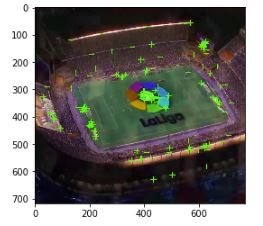
\includegraphics[width=8cm]{orb_simple_res.JPG}
\caption{Caractéristiques extraites par ORB (en vert), pour une seule image par plan}
\end{figure}
Ici, nous ne récupérons les caractéristiques que d'une seule image par transition de plan. L'image pour laquelle nous extrayons les caractéristiques est la dernière frame de la séquence, car c'est la dernière image faisant la transition entre deux plans (et dans le cas des logos, c'est dans celle-ci que sa forme visuelle est la plus nette).\\

L'algorithme est le suivant :\\
\begin{verbatim}
- S = les transition de plans détectées
- Récupérer le frame à la fin de chaque transition de plan dans S
  - nous obtenons |S| frame
- Pour chaque frame, calculer ses features (orb ou akaze)
  - Nous obtenons |S| vecteurs
- Utiliser KMeans avec K=2 pour séparer les vecteurs en deux groupes
  - le groupe le plus petit est le groupe des logo
\end{verbatim}

\subsubsection{Deuxième expérimentation : une séquence d'images par transition de plan:}
\label{sec:orgd90b786}
\begin{figure}[htbp]
\centering
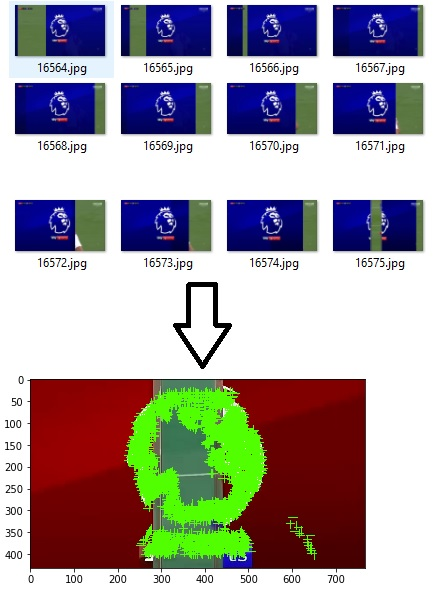
\includegraphics[width=8cm]{akaze_window_res.jpg}
\caption{Caractéristiques extraites par ORB (en vert) pour un séquence logo (agrégat des caractéristiques de chaque image dans le plan) \label{orb-window}}
\end{figure}
L'approche précédente ne récupère qu'une seule image par plan.\\
Or, le visuel des logos est présent sur plusieurs frames consécutifs.\\
Dans cette approche, nous récupérons plusieurs images consécutives pour chaque plan, et nous extrayons les caractéristiques pour chaque frame (voir figure \ref{orb-window}).\\

L'algorithme est le suivant :\\
\begin{verbatim}
- S = les transition de plans détectées
- Récupérer W frames pour chaque transition de plan dans S
  - nous obtenons |S| fenêtres de dimension W, où W est le nombre de frame
- Pour chaque fenêtre, calculer les features de chacun de ses frames (ORB)
  - Nous obtenons un vecteur de dimension S*W
- Utiliser KMeans avec K=2 pour séparer les vecteurs en deux groupes
  - le groupe le plus petit est le groupe des logos
\end{verbatim}

\subsection{Matching de contours}
\label{sec:org00fe23d}
Dans cette approche, nous allons chercher les frames qui ont des formes en commun dans la vidéo.\\
En effet, d'après l'hypothèse III, il est fort probable que si un frame à l'instant t a beaucoup de formes en commun avec un frame à l'instant t', avec \(2 < t' - t < 90\) (hypothèse V), alors il y a un logo à l'instant t et un logo à l'instant t', et un replay entre t et t'.\\

Dans cette méthode, nous utilisons là aussi le découpage en plan (\cite{Abd_Almageed_2008}).\\
Cet algorithme est particulièrement efficace dans notre cas, car les replays provoquent un changement de plan, les logos seront donc toujours à la transition entre deux plans. Cette méthode va nous permettre réduire la zone de recherche des logos aux frames qui font la transition entre deux plans.\\

L'idée est de chercher, pour chaque transition de plan, s'il existe une autre transition de plan dans son voisinage tel qu'ils ont des contours en commun dans plusieurs de leurs frames.\\

\subsubsection{Détection de contours}
\label{sec:orgee5191f}
\begin{figure}[htbp]
\centering
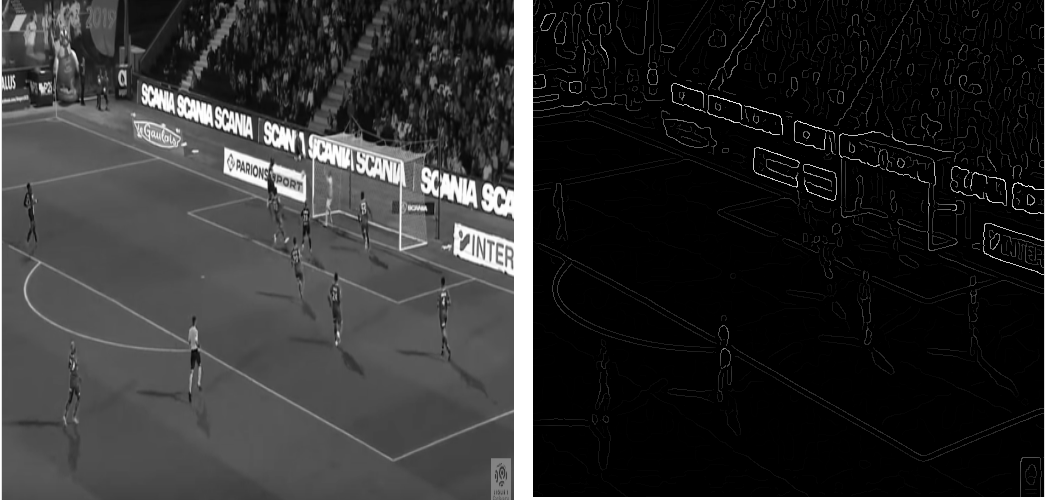
\includegraphics[width=10cm]{canny_edge2.png}
\caption{Détection de contours par filtre de Canny}
\end{figure}
Avec des algorithmes comme le filtre de Canny il est possible de détecter les contours des objets dans une image. Cet algorithme applique une opération de convolution sur les pixels de l'image. La matrice résultant de l'application de cette convolution est l'image décrivant les contours dans l'image source. Cet algorithme est sensible au bruit dans l'image, c'est pourquoi il est nécessaire d'opérer un lissage (par exemple un filtrage Gaussien) avant de l'appliquer.\\
L'intérêt de la détection de contours est de réduire l'information à traiter dans une image.\\

\subsubsection{Logos et contours}
\label{sec:orgf81f564}
\begin{figure}[htbp]
\centering
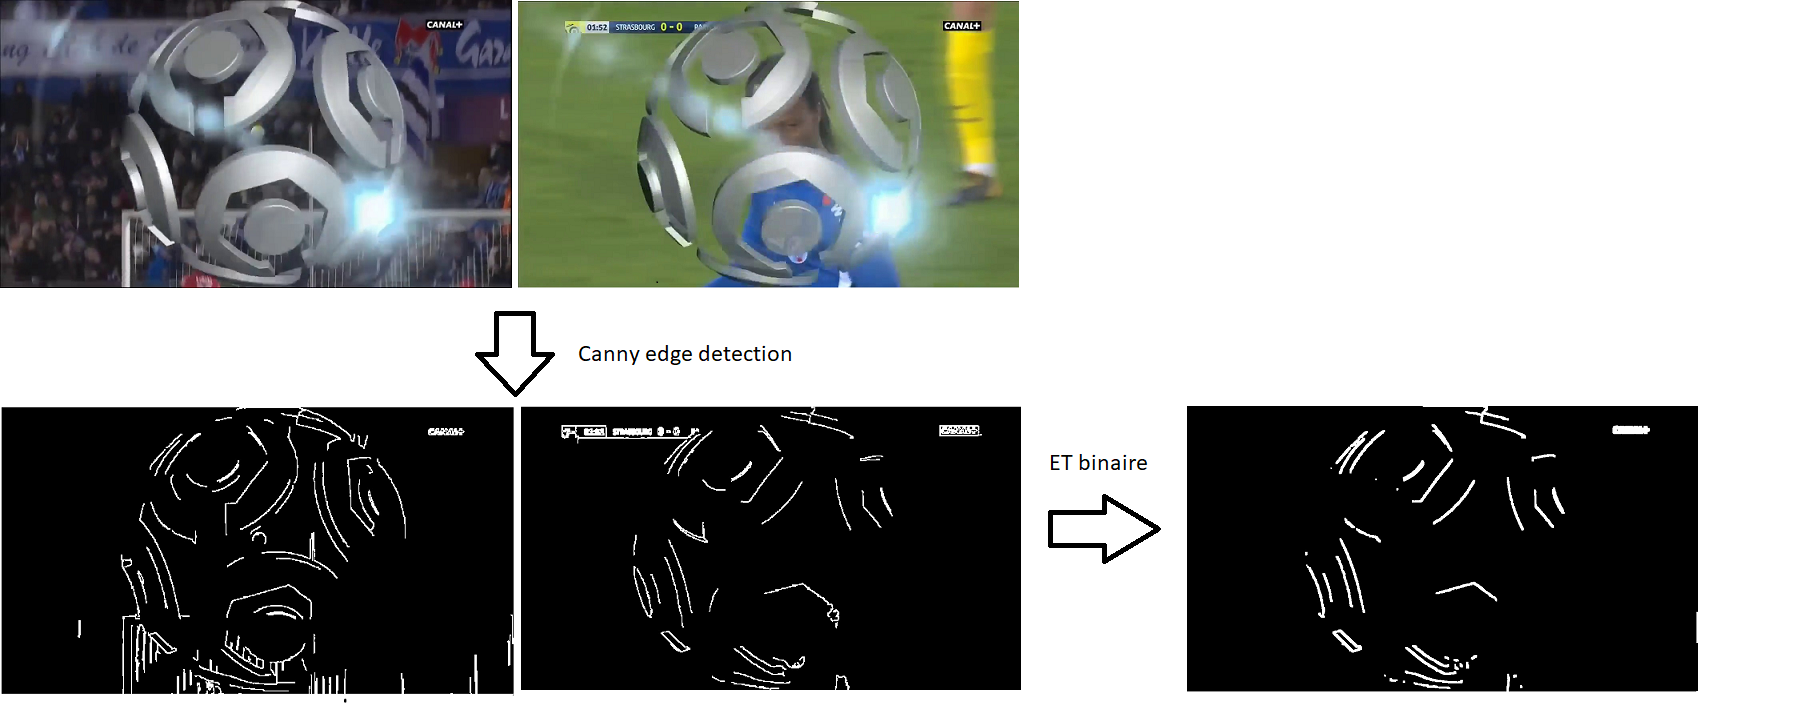
\includegraphics[width=10cm]{comparison_idea.png}
\caption{Comparaison des contours entre deux frames logos}
\end{figure}
\begin{figure}[htbp]
\centering
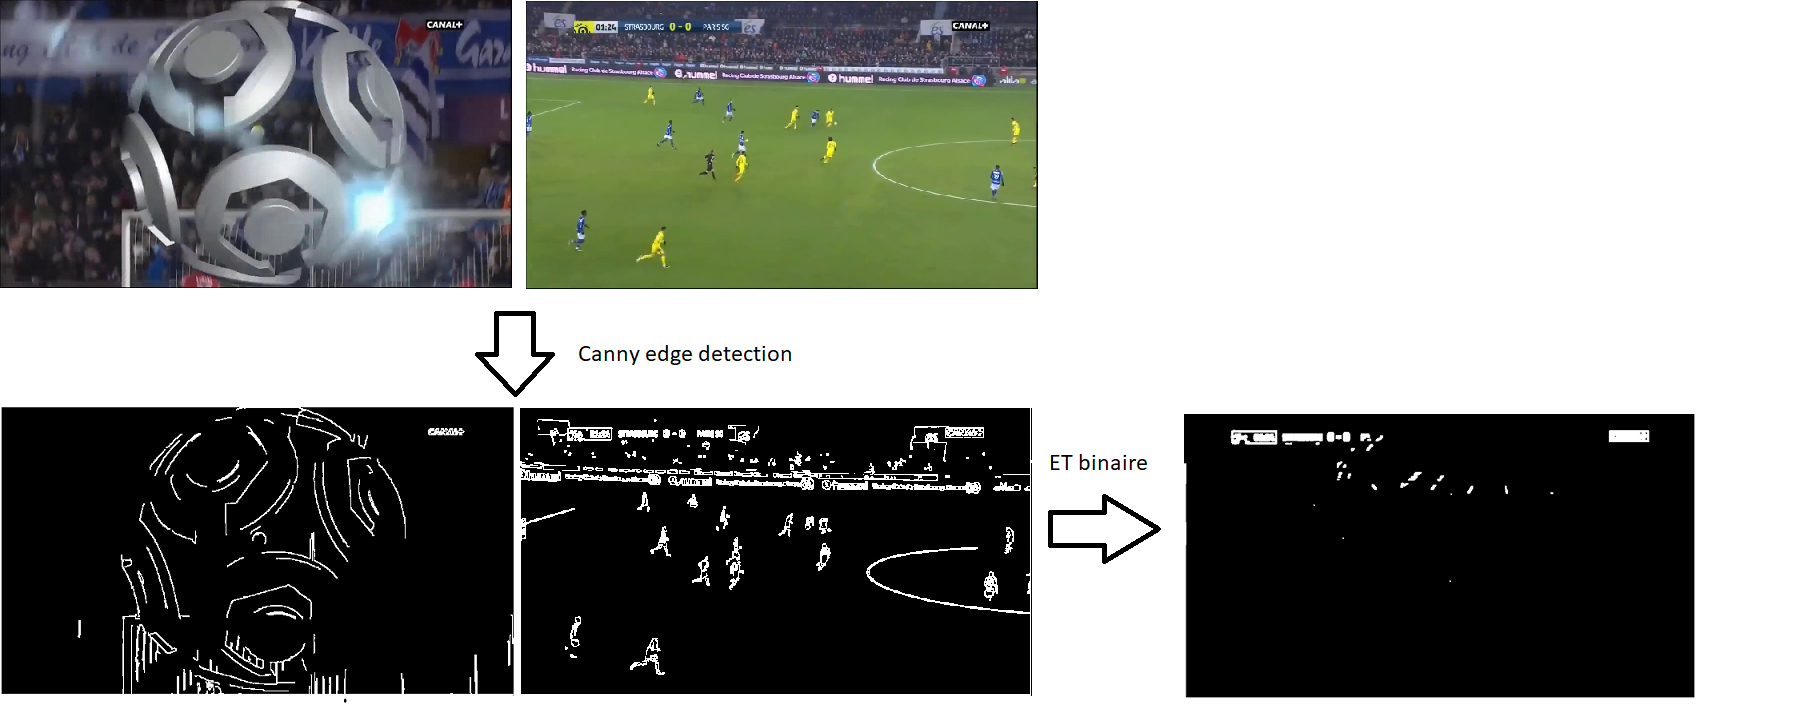
\includegraphics[width=10cm]{comparison_idea2.png}
\caption{Comparaison des contours entre une frame logo et une frame non logo}
\end{figure}

Les logos sont des séquences d'images incrustées dans la vidéo. En général, chaque séquence d'image logo est la même au pixel près que les autres séquences logos. Nécessairement, les contours détectés par filtre de Canny seront les mêmes. Pour savoir si deux images ont les mêmes contours, il suffit d'appliquer un ET binaire entre leur contour respectif, et de calculer la longueur des segments dans l'image résultant de ce ET binaire.\\
La longueur des segments nous donne un score, et si ce score est supérieur à un certain seuil, alors nous considérons que les deux images sont des logos.\\

\subsubsection{Mosaïque de plan}
\label{sec:org8968515}
\begin{figure}[htbp]
\centering
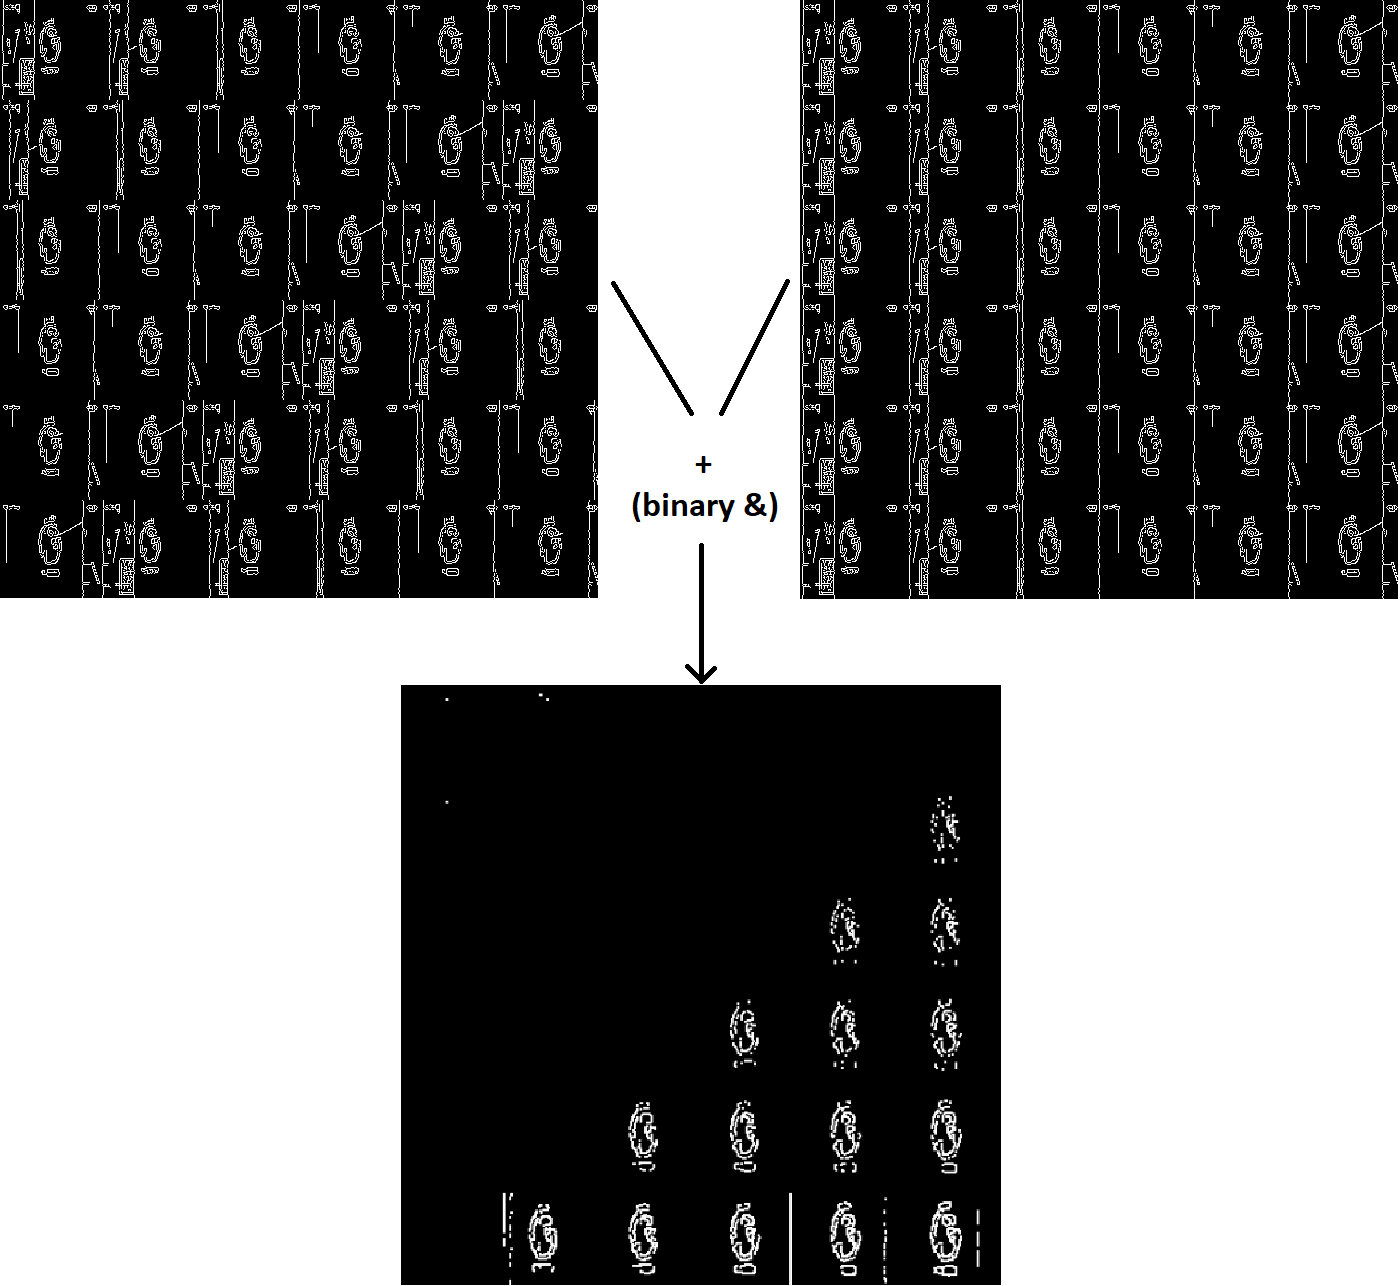
\includegraphics[width=16cm]{mosaique_add.png}
\caption{ET binaire (en bas) appliqué à une mosaïque de plan à l'instant t (à gauche) et à une mosaïque de plan à l'instant t' (à droite) \label{mosaic}}
\end{figure}
Pour des raisons d'optimisation, il n'est pas viable de comparer chaque frame de chaque transition de plan avec chaque frame des transitions voisines.\\
C'est pourquoi, pour chaque transition de plan, deux images sont générées.\\
Chaque image est de dimension (width * I) * (height*I) où I est le nombre de frames dans la transition. Chaque "case" dans l'image va correspondre aux contours d'une frame dans la transition de plan.\\
La première matrice a un décalage d'un frame par ligne, la seconde n'a pas de décalage.\\
Pour comparer deux shot (figure \ref{mosaic}), il suffit d’appliquer un ET binaire entre les matrices des mosaïques, puis de calculer la longueur des contours dans cette matrice (les images sont des matrices).\\
L'idée derrière la mosaïque de plan est d'avoir les contours pour toutes les images de la transition de plan dans une même image.\\

\subsubsection{Algorithme}
\label{sec:org83b6e19}
\begin{verbatim}
- Pré traitement sur les images
  1. Redimensionner chaque image
  2. Cropper chaque image (afin de supprimer certains faux positifs)
  3. Détecter le contour (par filtre de Canny)
- Génération des mosaïques
- Pour chaque mosaïque de plan S_A :
  - Pour chaque mosaïque de plan S_B après S_A :
    1. Contour_commun = C_A & C_B
    2. Contours_diff = Détection des contours de Contour_commun
    3. Résultat = Ne garder que les contours qui sont assez longs (|contours| > K)
    4. Si Résultat > Seuil : alors S_A et S_B sont des logos potentiels
- Pour chaque logo potentiel LP :
  1. Le comparer avec les autres logo L’ (même procédure qu’en 2)
  2. Si au moins 2 logos L’  match, alors LP est un logo
- Trouver les replays grâce aux logos
\end{verbatim}

Notre algorithme est sensible au plan fixe et aux images avec beaucoup de bruits (ces images ont beaucoup de contours détectés par l’algorithme de détection de contours).\\
Beaucoup de ces faux-positifs peuvent être filtrés lors du pré-traitement sur les plans, notamment en rajoutant du blur, néanmoins, nous ne sommes pas parvenus à filtrer 100\% des faux-positifs.\\

\subsection{Convolution 3D sur des séquences d'images}
\label{sec:orge16e0d8}
Dans cette approche, nous allons implémenter une méthode similaire à \cite{Tran_2015}.\\
L'idée va être d'entraîner un réseau à convolution avec une couche de convolution 3D.\\
Cette couche va prendre en entrée une séquence d'images et va prédire une classe logo ou non-logo.\\
Pour réduire la zone de recherche, seulement les séquences d'images entre deux plans (détectées avec \cite{Abd_Almageed_2008}) seront traitées.\\
Lors de l'entraînement, le réseau va apprendre à partir de séquences d'images labellisées (logo/non-logo).\\
Comme pour \cite{Tran_2015}, nous pensons que la convolution 3D va permettre au réseau d'apprendre l'apparence des logos mais aussi leur animation dans la vidéo.\\

\subsection{Convolution 3D sur des séquences d'images de flux optique}
\label{sec:org7eea183}
Dans cette approche, nous allons entraîner un classifieur de séquences d'images de flux optique.\\
Nous pensons que, comme pour l'approche par convolution 3D sur les séquences d'images logos/non-logos, la convolution 3D va permettre d'apprendre le déplacement des objets dans le temps. La troisième dimension du réseau est la temporalité, et les deux autres sont la composante spatiale modélisée par les images de flux optiques.\\
Lors de l'entraînement, le réseau va apprendre à partir de séquences d'images de flux optique labellisées (logo/non-logo).\\
Là aussi, nous n'allons traiter que les frames qui sont entre deux plans (\cite{Abd_Almageed_2008}).\\

\newpage
\section{Collecte des données \& entraînement}
\label{sec:orgdfabe6f}
\subsection{Ensemble de données}
\label{sec:org7257dac}
L'objectif de la collecte de données est d'obtenir les ensembles de données suivants :\\
\begin{itemize}
\item Dataset non logo\\
\item Dataset logo\\
\end{itemize}
Chaque élément de l'ensemble de données contient :\\
\begin{itemize}
\item une séquence de 20 images labellisée logo ou non logo (pour un classifieur d'image à convolution 3D)\\
\item une séquence de 19 images de flux optique labellisée logo ou non logo (pour un classifieur de flux optique à convolution 3D)\\
\end{itemize}

\subsection{Collecte des données}
\label{sec:org371e7be}
L'approche par matching de contours convient tout à fait pour former notre ensemble de données de logo.\\

En effet, elle est :\\
\begin{itemize}
\item rapide : une vidéo au format 100x100 de 200000 frames va être traitée en moins de cinq minutes, et en moyenne une cinquentaine de logos (séquence d'images pendant laquelle un logo apparaît) sont extraits par vidéo\\
\item précise : il est possible de modifier les paramètres pour que l'algorithme ne renvoie presque pas de faux-positifs (>1\%)\\
\end{itemize}

\subsection{Obtention des images de flux optiques}
\label{sec:orgb0858ea}
Pour obtenir les images de flux optiques, nous allons utiliser notre algorithme de détection de logo par matching de contours afin d'obtenir les séquences d'images comprises entre deux plans.\\
L'algorithme va récupérer des séquences d'images logos/non-logos. Pour obtenir une séquence d'images de flux optique à partir de ces séquences, il suffit de calculer le flux optique entre une frame et la frame suivante; ainsi, nous obtenons une matrice de dimension 2, et donc une image.\\
Dans notre cas, les séquences d'images sont de taille 20, donc les séquences d'images de flux optique sont de taille 19.\\

\subsection{Architecture du scrapper}
\label{sec:orgc85495f}
\begin{figure}[htbp]
\centering
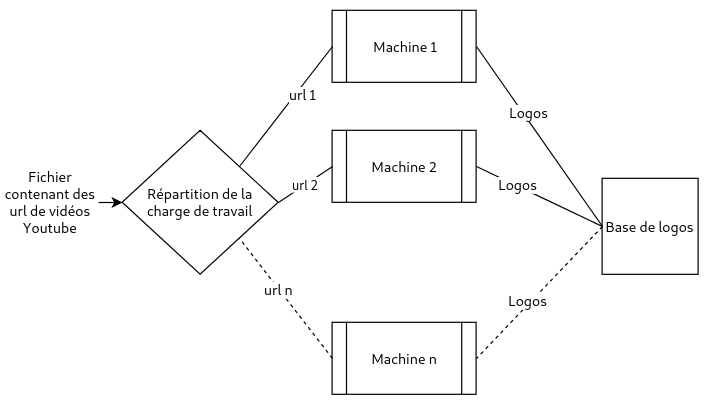
\includegraphics[width=15cm]{arch_scrap.png}
\caption{Architecture du scrapper de logos \label{arch-scrap}}
\end{figure}
Nous voulons une architecture de \emph{scrapping} qui soit distribuée. Cette architecture est présentée dans la figure \ref{arch-scrap}.\\
En effet, le traitement d'une vidéo prend en moyenne trente minutes (10 minutes pour trouver les replays, et 20 minutes pour l'import des fichiers etc..), il est donc nécessaire de pouvoir traiter plusieurs vidéos en même temps.\\
Pour mettre en place cette architecture, nous avons créé une image \emph{Docker} englobant le programme de détection de logos par matching de contours et qui importe les frames des séquences logo ainsi que leur flux optique sur la solution de stockage de GCP (storage).\\
L'image est stockée sur le Container Registry de GCP, et va être lancée dans un container.\\

\subsubsection{Kubernetes}
\label{sec:org978028d}
\begin{figure}[htbp]
\centering
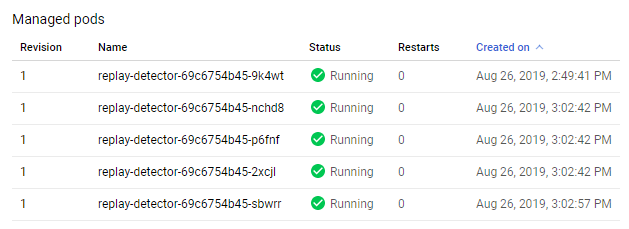
\includegraphics[width=10cm]{kubernetes_pods.PNG}
\caption{Cluster Kubernetes sur GCP \label{cluster-kubernetes}}
\end{figure}
Un \emph{cluster} Kubernetes \ref{cluster-kubernetes} avec un \emph{load balancer} va se charger d'ordonner les containers et de repartir la charge de travail entre les différents "pods" (unité exécutant un conteneur Docker).\\
Ainsi, il va être possible de traiter plusieurs vidéos en même temps car la charge de travail ne sera plus répartie sur une seule machine, mais sur plusieurs. Kubernetes est un outil efficace de mise à l'échelle.\\
\subsection{Données collectées}
\label{sec:org56eef65}
Nous avons parsé plusieurs vidéos de matchs de football. Au total, 2611 séquences de logos et 2611 séquences non-logo ont été obtenues.\\
En tout, plus de 200000 images sont générées (8 go sur disque) :\\
\begin{itemize}
\item 2611 séquences de 20 images non-logos\\
\item 2611 séquences de 20 images logos\\
\item 2611 séquences de 19 images de flux optique non-logos\\
\item 2611 séquences de 19 images de flux optique logos\\
\end{itemize}

\subsection{Entraînement et architectures des modèles}
\label{sec:orga489303}
L'entraînement va se faire en utilisant les instances de machines virtuelles préconfigurées pour l'apprentissage profond de Google Cloud. Le framework utilisé est Keras.\\
Pour entraîner les réseaux à convolution 3D (classifieur de séquences d'images et classifieur de séquences d'images de flux optique), nous allons reprendre l'architecture proposée par \cite{Tran_2015}.\\

Le ratio ensemble d'entraînement/ensemble de validation est de 0,8.\\

\subsubsection{Entraînement du classifieur de séquences d'images}
\label{sec:orgdcc5b69}
\begin{figure}[htbp]
\centering
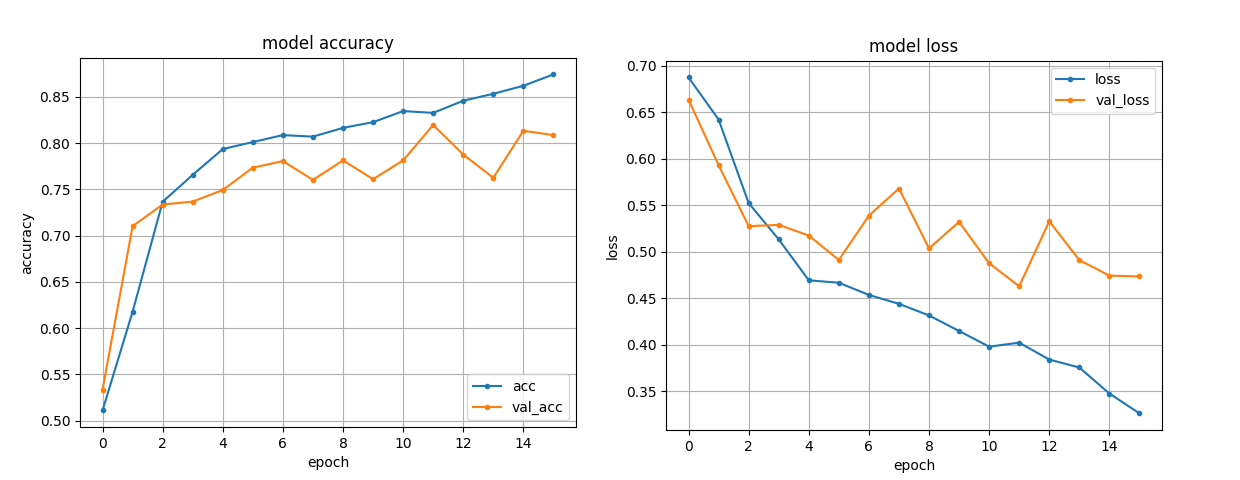
\includegraphics[width=10cm]{conv_train.png}
\caption{Entraînement du classifieur de séquence d'images}
\end{figure}
Nous voyons que le minima de la fonction de perte (val\(_{\text{loss}}\)) est atteint après 11 epoch (0,46), la précision (val\(_{\text{acc}}\)) sur l'ensemble de test après 11 epoch est de 82\%.\\
\subsubsection{Entraînement du classifieur de séquences d'images de flux optique}
\label{sec:org7301e1b}
\begin{figure}[htbp]
\centering
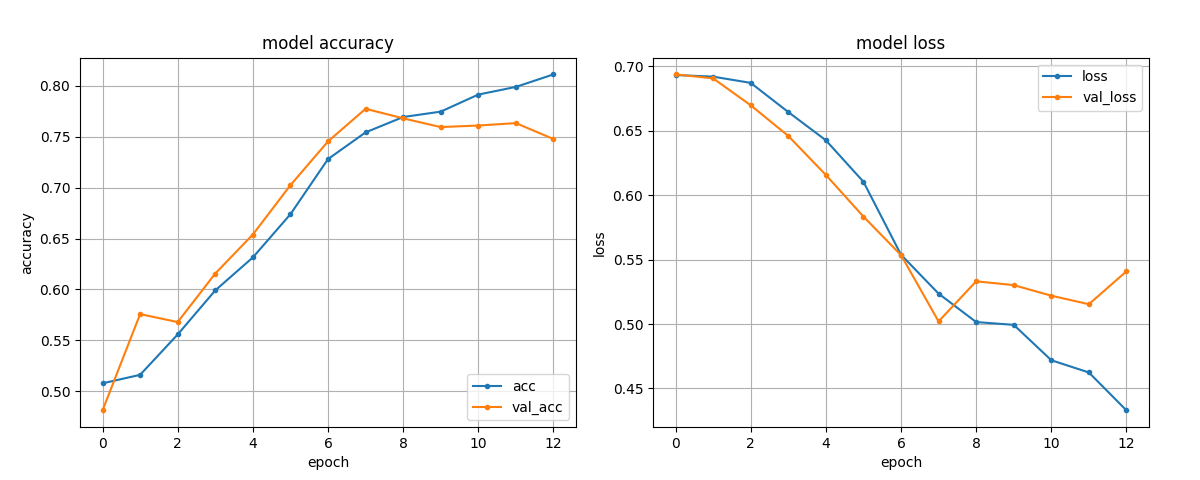
\includegraphics[width=10cm]{flow_train.png}
\caption{Entraînement du classifieur de séquence d'images de flux optique}
\end{figure}
Le minima de la fonction de perte (val\(_{\text{loss}}\)) est atteint après 7 epoch (0,50), pour une précision (val\(_{\text{acc}}\)) de 77\% sur l'ensemble de test.\\

\subsection{Difficultés rencontrées}
\label{sec:org1a261a8}
\subsubsection{Avoir une machine assez puissante pour la convolution 3D}
\label{sec:org87d061a}
L'entraînement n'est pas possible sur une machine non dotée d'une carte graphique puissante. Pour ça, nous avons du utilisé une machine virtuelle fournie par Google. L'inconvénient de cette solution est le prix. En effet, celle-ci coûte près de 300€ par mois; ce qui ne nous a permis d'essayer autant de modèle qui nous aurions aimé, car l'entraînement est long et donc coûteux.\\
\subsubsection{La gestion de l'ensemble de données}
\label{sec:org4e19863}
Pour 2611 exemples de séquences logo et 2611 exemples de séquences non-logo, la taille de l'ensemble de données atteint presque les 10go pour plus de 200000 images. Pour archiver ces images, nous avons opté pour la structure arborescente suivante : tag/type-image/id-séquence/images-séquences; où tag peut être logo ou non logo, type-image peut être flux optique ou normal (séquence de frame dans la vidéo), id-séquence un identifiant unique associé à chaque séquence et images-séquences les images de la séquence.\\
Manipuler autant de données est un problème complexe à bien des niveaux : l'importation/exportation des fichiers est longue (surtout le déplacement de ceux-ci entre la machine locale et la machine à distance), réorganiser la structure des dossiers est compliqué en cas d'erreur, les données erronnées (par exemple si le dossier représentant une séquence est vide suite à une défaillance du scrapper) sont difficilement détectables, l'extraction de l'archive contenant le dataset prend du temps, etc\ldots{} À titre d'exemple, même sur la machine très puissante fournie par Google, l'extraction de l'archive contenant toutes les images de notre ensemble de données prend plus d'une heure.\\
\subsubsection{Adaptation des données pour le réseau}
\label{sec:org1520b98}
Les données sont des dossiers contenant des séquences d'images logo/non-logo.\\
Pour pouvoir donner en entrée ces données aux réseaux, nous avons besoin de transformer les séquences d'images en vecteur de dimension 4 (nombres d'images, largeur de chaque image, longueur de chaque image et nombre de canaux de chaque image) et de faire en sorte de pouvoir donner ces vecteurs en entrée du réseau par batch. La solution a ce problème a été de créer un \emph{generator} personnalisé qui se charge d'aller lire les séquences dans le bon dossier et de ne charger en mémoire que le nombre nécessaire de séquences (taille du batch).\\

\newpage
\section{Résultats obtenus}
\label{sec:org72ead63}
Dans cette partie, nous allons évaluer chaque approche sur le même ensemble d'évalutation.\\

\subsection{Procédure d'évaluation}
\label{sec:org0da0648}
L'ensemble d'évaluation est le suivant : une vidéo de Ligue 1 de 150k frames, une vidéo de Ligue 1 de 80k frames, une vidéo de Liga et enfin une vidéo de Premier League. Trois logos différents (Liga, Ligue 1 et Premier League) vont servir à évaluer nos approches.\\
Dans toutes les expérimentations, la vidéo est découpée en plans et nous récupérons les transitions de plan. L'évaluation porte sur le nombre de logos correctement détectés dans la vidéo.\\

\subsection{Résultats pour ORB}
\label{sec:org471d6af}
\begin{figure}[htbp]
\centering
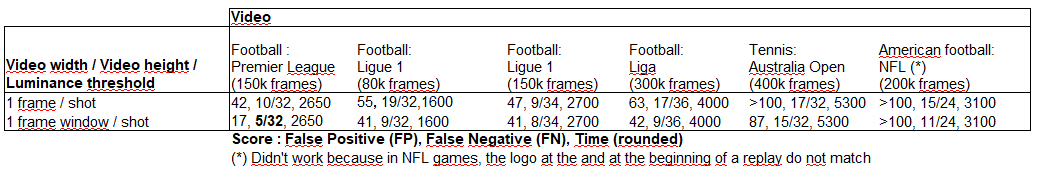
\includegraphics[width=15cm]{res_orb.png}
\caption{Résultats obtenus pour le clustering avec les caractéristiques extraites par ORB \label{orb-res}}
\end{figure}

Les résultats sont présentés dans la figure \ref{orb-res}. Cette approche à tendance à considérer trop de séquences comme des séquences logos (faible précision sur toutes les vidéos).\\
Le gros inconvénient de cette méthode est le caractère arbitraire de la sélection du groupe de logo après le clustering.\\
En effet, nous faisons l'hypothèse qu'il y aura toujours plus de non-logos que de logos, ce qui n'est pas toujours vrai.\\
De plus, l'algorithme d'extraction de caractéristiques ne marche pas toujours très bien, ce qui fausse évidemment le clustering par la suite.\\

Néanmoins, il est intéressant de remarquer que les résultats avec la fenêtre de frame sont toujours meilleurs que les résultats avec un seul frame.\\

\subsection{Résultats pour l'approche par matching de contours}
\label{sec:org27dd034}
\begin{figure}[htbp]
\centering
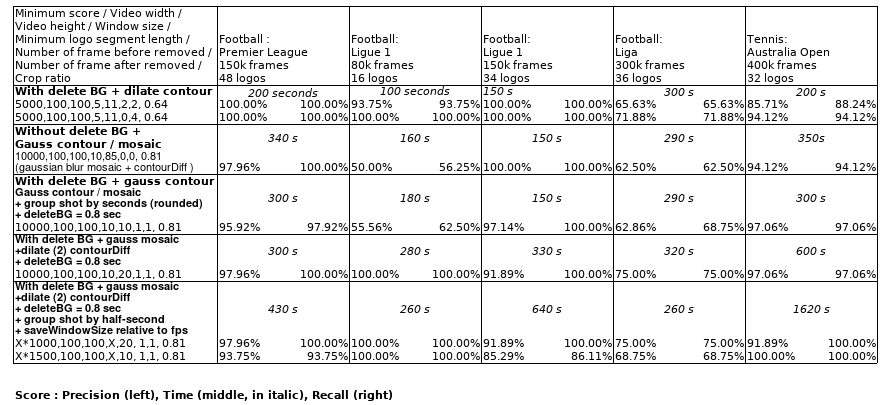
\includegraphics[width=17cm]{res_match_contour.png}
\caption{Résultats obtenus \label{res-match-contour}}
\end{figure}
Les résultats obtenus sont présentés en \ref{res-match-contour}. Chaque ligne correspond à une configuration de paramètres différente, les paramètres sont :\\
\begin{itemize}
\item With delete BG : lors de la création de la mosaïque de plan, nous faisons pour chaque frame de la mosaïque la soustraction entre ce frame et les 3 frames au début du plan. Nous faisons ceci afin de supprimer les pixels fixes dans le plan qui sont probablement du bruit, comme par exemple, les lignes du terrain, les cages du gardien ou le logo de la chaine. En effet, les frames avec des pixels fixes vont avoir beaucoup de contours en commun et risque donc d'être détectées comme logo sans l'être.\\
\item dilate contour : les pixels des contours sont dilatés (de 2 pixels)\\
\item gauss contour/mosaic : un filtre gaussien est appliqué sur la matrice résultant du \& binaire entre deux mosaïques de contours de plan.\\
\item saveWindowSize relative to fps : la taille des mosaïques est relative au nombre d'images par seconde dans la vidéo\\
\end{itemize}

Après avoir fait plusieurs essais avec des paramètres différents à chaque fois, nous ne sommes pas parvenus à trouver une combinaison telle qu'il n'y ait aucun faux positif et aucun faux négatif.\\

Concernant le temps d’exécution, celui-ci est relié presque entièrement à la taille de la vidéo donnée en entrée, ainsi qu’à la taille des mosaïques. Il reste néanmoins faible, et cette approche peut être utilisée en temps réel.\\

L'inconvénient de cette méthode est qu'elle n'est pas capable de détecter les replays dans les cas suivants :\\
\begin{itemize}
\item s'il n’y a pas de logo pour les replays (simple fondu)\\
\item si les logos au début et à la fin des replays ne sont pas les mêmes\\
\item s'il y a des logos au début des replays, mais pas de logo à la fin des replays (un simple fondu remplace le logo).\\
\end{itemize}

\subsection{Résultats pour l'approche par apprentissage profond}
\label{sec:orgc7252f1}
\begin{figure}[htbp]
\centering
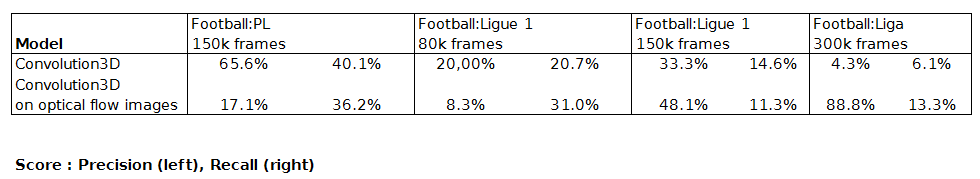
\includegraphics[width=15cm]{res_conv.png}
\caption{Résultats obtenus par les réseaux \label{conv-res}}
\end{figure}
Les résultats obtenus par les réseaux sont présentés en \ref{conv-res}. Ils sont moins bons que ce que nous espérions.\\
Le réseau à convolution 3D sur des séquences d'images obtient des résultats satisfaisant sur la vidéo de Premier League (PL) avec 65\% de précision et 40\% de rappel; mais de mauvais résultats sur les autres vidéos.\\
Le réseau à convolution 3D sur des séquences d'images de flux optique obtient de mauvais résultats sur toutes les vidéos; le résultat obtenu pour la vidéo de Liga est néanmoins intéressant. En effet, avec une précision de 88\%, il semblerait que le réseau ait commencé à apprendre à reconnaître les séquences non-logo.\\

Les possibles raisons pouvant expliquer ces mauvais résultats sont les suivantes :\\
\begin{itemize}
\item les données d'entraînement ne sont pas assez représentatives (I) : l'ensemble d'entraînement est constitué de 50\% de séquences logos et de 50\% de séquences non logos alors que dans les faits, seulement 5\% en moyenne des séquences dans les matchs de football sont des séquences logos. Nous avons procédé ainsi pour avoir un ensemble de données plus petit que si nous avions gardé toutes les séquences non-logos (le dataset aurait été près de 5 fois plus volumineux)\\
\item les données d'entraînement ne sont pas assez représentatives (II) : la majorité des séquences logos (\textasciitilde{}90\%) que nous avons dans l'ensemble d'entraînement sont des logos de Liga. Ceci est du au fait que la plupart des vidéos que nous avons pu récupérer sont des vidéos de Liga.\\
\item les données d'entraînement ne sont pas d'assez bonne qualité : certaines vidéos sont de mauvaise qualité et même dans certains cas les logos sont floutés\\
\item le scrapper n'est pas parfait : l'annotation logo/non-logo des séquences est automatique. Il est probable qu'une quantité non négligeable de séquences soient incorrectement annotées.\\
\item l'ensemble de données est trop petit : nous entraînons les réseaux "de zéro", il est probable que 2000 séquences logos et 2000 séquences non-logos ne suffisent pas. Nous avons fait le choix de garder l'ensemble d'entraînement à 4000 exemples car un dataset plus gros aurait accru le temps d'entraînement (et donc le coût de la machine distante).\\
\end{itemize}

\newpage
\section{Conclusion}
\label{sec:org8156e54}
L'approche la plus efficace pour la détection de replays est l'approche par détection de contours. En effet, celle-ci obtient les meilleurs résultats sur toutes les vidéos d'évaluation. De plus, elle est la plus rapide et n'est pas coûteuse en terme de puissance de calcul : les calculs se font sur le processeur (et non pas sur carte graphique comme les approches par apprentissage profond) et il faut seulement une vingtaine de minutes pour analyser 200000 frames sur un processeur Intel(R) Core(TM) i5-2520M CPU @ 2.50GHz. Il est donc possible d'utiliser cette méthode en temps réel.\\
Néanmoins, l'approche par détection de contours présente des inconvénients. Le premier est qu'elle est trop sensible aux bruits dans les vidéos. Le second est la trop forte dépendance aux hyper-paramètres (taille en pixel des images, nombre de frames dans la mosaïque, paramètres du floutage gaussien, \ldots{}). Le dernier est que cette approche ne parviendra jamais à détecter certaines séquences logos, comme par exemple les logos qui ne sont pas les mêmes au début d'un replay et à la fin d'un replay.\\
Ces inconvénients s'expliquent par le fait que cette méthode n'est pas \emph{adaptative} car elle n'apprend pas ce qu'est une séquence logo.\\
Même si les résultats obtenus par les réseaux ne sont pas excellents, ils ne sont pas affectés par les trois inconvénients cités plus haut.\\
Les résultats obtenus pour la vidéo de Premier League nous laissent penser que le réseau \emph{a commencé} à apprendre la forme des séquences non logos dans les vidéos.\\
Il serait intéressant de reprendre cette étude, avec cette fois-ci un ensemble de données à la fois plus conséquent et plus propre (avec de l'annotation humaine).\\
Une autre piste à étudier est le \emph{transfer learning}. Dans notre cas, nous pouvons utiliser les poids appris par les auteurs du réseau C3D sur le dataset UCF101 \cite{Tran_2015}. Il serait aussi intéressant d'étudier d'autres modèles comme celui mélant LSTM et CNN \cite{Joe_Yue_Hei_Ng_2015}.\\
Pour conclure sur cette recherche, nous dirons que l'analyse vidéo n'est pas chose aisée. Entraîner un classifieur pour cette tâche demande des machines très performantes ainsi qu'un ensemble de données très riches.\\
Il est important de préciser que la complexité croit de manière exponentielle avec la taille de l'ensemble de données. Par exemple, changer la convention de nommage des exemples d'entraînement n'est pas le même problème si le dataset fait 500mo ou 10go. Une grande partie de notre travail a consisté à ré-organiser l'ensemble de données et à retrouver des exemples défaillants parmi la grande quantité d'images.\\

\newpage
\section{Glossaire}
\label{sec:org0d18543}
\begin{itemize}
\item Batch : un groupe d'échantillon d'entraînement; permet de traiter l'ensemble d'apprentissage plus vite qu'en ne traitant qu'un seul échantillon à la fois.\\
\item Clustering : procédé permettant de regrouper des éléments\\
\item Histogramme : représentation d'une image en fonction de ses canaux de couleurs (rouge, vert, bleu)\\
\item Frame : une image à l'instant t d'une vidéo\\
\item Shot : un plan\\
\item FPS : frame per second / image par seconde\\
\item Cropper : sélectionner une partie continue des pixels l'image\\
\item RNN : Recurrent Neural Networks, ou réseaux de neurones récurrents (RNR) en français\\
\item CNN : Convolutional Neural Network, réseaux de neurones convolutifs (RNC) en français\\
\item LSTM : Long Short Term Memory\\
\item Cluster : un groupe; en apprentissage automatique, signifie un groupe d'objet partageant des caractèristiques similaires; en infrastructure réseau, signifie un ensemble de machines\\
\item Scrapping : technique d'extraction de contenu de sites Web; dans notre cas, nous récupérons des vidéos sur Youtube\\
\item Transfer learning: procédé d'apprentissage automatique consistant à réutiliser les poids appris par un réseau dans un autre réseau\\
\item Slow motion : nous parlons de slow-motion quand les objets se déplacent moins vite que la normale dans une vidéo\\
\item Docker : solution permettant de lancer une application dans son propre environnement (image) à partir d'une suite d'instruction (Dockerfile)\\
\item GCP : Google Cloud Platform\\
\item Load balancer : technique permettant de répartir la charge de travail parmi un ensemble de machines\\
\item Framework : ensemble de librairies facilitant la tâche du programmeur\\
\item Dataset : anglicisme fréquemment utilisé pour parler d'un ensemble de données\\
\end{itemize}

\newpage
\section{Table des figures}
\label{sec:orgc72f010}
\ref{calc-dist} Xu, W., \& Yi, Y., A robust replay detection algorithm for soccer video, IEEE Signal Processing Letters, 18(9), 509–512 (2011).  \url{http://dx.doi.org/10.1109/lsp.2011.2161287}. Equation (4)\\

\ref{mean-shift-res} Duan, L., Xu, M., Tian, Q., \& Xu, C., Mean shift based video segment representation and applications to replay detection, 2004 IEEE International Conference on Acoustics, Speech, and Signal Processing, (),  ().  \url{http://dx.doi.org/10.1109/icassp.2004.1327209}. Table 1\\

\ref{sparse-vs-dense} Goodfellow, I., Bengio, Y., \& Courville, A., Deep Learning (2016), : MIT Press. \cite{Goodfellow-et-al-2016} Figure 9.2\\

\ref{optical-flow} Simonyan, K., \& Zisserman, A., Two-stream convolutional networks for action recognition in videos, CoRR, abs/1406.2199(),  (2014). Figure 2\\

\ref{c3d-res} Tran, D., Bourdev, L., Fergus, R., Torresani, L., \& Paluri, M., Learning spatiotemporal features with 3d convolutional networks, 2015 IEEE International Conference on Computer Vision (ICCV), (),  (2015).  \url{http://dx.doi.org/10.1109/iccv.2015.510}. Table 3\\

\ref{opt-flow} Simonyan, K., \& Zisserman, A., Two-stream convolutional networks for action recognition in videos, CoRR, abs/1406.2199(),  (2014). Figure 2\\

\ref{two-stream-res} Simonyan, K., \& Zisserman, A., Two-stream convolutional networks for action recognition in videos, CoRR, abs/1406.2199(),  (2014). Table 4\\

\ref{arch-c3d} Tran, D., Bourdev, L., Fergus, R., Torresani, L., \& Paluri, M., Learning spatiotemporal features with 3d convolutional networks, 2015 IEEE International Conference on Computer Vision (ICCV), (),  (2015).  \url{http://dx.doi.org/10.1109/iccv.2015.510}. Figure 3\\

\ref{arch-lstm} Ng, J. Y., Hausknecht, M., Vijayanarasimhan, S., Vinyals, O., Monga, R., \& Toderici, G., Beyond short snippets: deep networks for video classification, 2015 IEEE Conference on Computer Vision and Pattern Recognition (CVPR), (),  (2015).  \url{http://dx.doi.org/10.1109/cvpr.2015.7299101}. Figure 4\\

\ref{convolution} Goodfellow, I., Bengio, Y., \& Courville, A., Deep Learning (2016), : MIT Press. Chapitre 9. Figure 9.1\\

\ref{pooling} Goodfellow, I., Bengio, Y., \& Courville, A., Deep Learning (2016), : MIT Press. Chapitre 9. Figure 9.9\\

\ref{c3d-idea} Tran, D., Bourdev, L., Fergus, R., Torresani, L., \& Paluri, M., Learning spatiotemporal features with 3d convolutional networks, 2015 IEEE International Conference on Computer Vision (ICCV), (),  (2015).  \url{http://dx.doi.org/10.1109/iccv.2015.510}. Figure 1\\

\ref{cnn_lstm} Ng, J. Y., Hausknecht, M., Vijayanarasimhan, S., Vinyals, O., Monga, R., \& Toderici, G., Beyond short snippets: deep networks for video classification, 2015 IEEE Conference on Computer Vision and Pattern Recognition (CVPR), (),  (2015).  \url{http://dx.doi.org/10.1109/cvpr.2015.7299101}. Table 7\\
\bibliographystyle{unsrt}
\bibliography{summary}
\end{document}
